\documentclass[]{elsarticle} %review=doublespace preprint=single 5p=2 column
%%% Begin My package additions %%%%%%%%%%%%%%%%%%%
\usepackage[hyphens]{url}

  \journal{European Journal of Operational Research} % Sets Journal name


\usepackage{lineno} % add
\providecommand{\tightlist}{%
  \setlength{\itemsep}{0pt}\setlength{\parskip}{0pt}}

\usepackage{graphicx}
%%%%%%%%%%%%%%%% end my additions to header

\usepackage[T1]{fontenc}
\usepackage{lmodern}
\usepackage{amssymb,amsmath}
\usepackage{ifxetex,ifluatex}
\usepackage{fixltx2e} % provides \textsubscript
% use upquote if available, for straight quotes in verbatim environments
\IfFileExists{upquote.sty}{\usepackage{upquote}}{}
\ifnum 0\ifxetex 1\fi\ifluatex 1\fi=0 % if pdftex
  \usepackage[utf8]{inputenc}
\else % if luatex or xelatex
  \usepackage{fontspec}
  \ifxetex
    \usepackage{xltxtra,xunicode}
  \fi
  \defaultfontfeatures{Mapping=tex-text,Scale=MatchLowercase}
  \newcommand{\euro}{€}
\fi
% use microtype if available
\IfFileExists{microtype.sty}{\usepackage{microtype}}{}
\usepackage[top=25mm, left=30mm, right=30mm, bottom=25mm,headsep=10mm,
footskip=12mm]{geometry}
\bibliographystyle{elsarticle-harv}
\ifxetex
  \usepackage[setpagesize=false, % page size defined by xetex
              unicode=false, % unicode breaks when used with xetex
              xetex]{hyperref}
\else
  \usepackage[unicode=true]{hyperref}
\fi
\hypersetup{breaklinks=true,
            bookmarks=true,
            pdfauthor={},
            pdftitle={On time series features and forecasting by temporal aggregation},
            colorlinks=false,
            urlcolor=blue,
            linkcolor=magenta,
            pdfborder={0 0 0}}
\urlstyle{same}  % don't use monospace font for urls

\setcounter{secnumdepth}{5}
% Pandoc toggle for numbering sections (defaults to be off)

% Pandoc citation processing
\newlength{\cslhangindent}
\setlength{\cslhangindent}{1.5em}
\newlength{\csllabelwidth}
\setlength{\csllabelwidth}{3em}
% for Pandoc 2.8 to 2.10.1
\newenvironment{cslreferences}%
  {}%
  {\par}
% For Pandoc 2.11+
\newenvironment{CSLReferences}[2] % #1 hanging-ident, #2 entry spacing
 {% don't indent paragraphs
  \setlength{\parindent}{0pt}
  % turn on hanging indent if param 1 is 1
  \ifodd #1 \everypar{\setlength{\hangindent}{\cslhangindent}}\ignorespaces\fi
  % set entry spacing
  \ifnum #2 > 0
  \setlength{\parskip}{#2\baselineskip}
  \fi
 }%
 {}
\usepackage{calc}
\newcommand{\CSLBlock}[1]{#1\hfill\break}
\newcommand{\CSLLeftMargin}[1]{\parbox[t]{\csllabelwidth}{#1}}
\newcommand{\CSLRightInline}[1]{\parbox[t]{\linewidth - \csllabelwidth}{#1}\break}
\newcommand{\CSLIndent}[1]{\hspace{\cslhangindent}#1}

% Pandoc header
\usepackage{float}
\floatplacement{figure}{!htb}
\usepackage{algorithm}
\usepackage{algpseudocode}
\usepackage{enumitem}
\usepackage{pdflscape}
\newcommand{\blandscape}{\begin{landscape}}
\newcommand{\elandscape}{\end{landscape}}
\usepackage{booktabs}
\usepackage{longtable}
\usepackage{array}
\usepackage{multirow}
\usepackage{wrapfig}
\usepackage{float}
\usepackage{colortbl}
\usepackage{pdflscape}
\usepackage{tabu}
\usepackage{threeparttable}
\usepackage{threeparttablex}
\usepackage[normalem]{ulem}
\usepackage{makecell}
\usepackage{xcolor}



\begin{document}
\begin{frontmatter}

  \title{On time series features and forecasting by temporal
aggregation}
    \author[Cardiff Business School]{Bahman Rostami-tabar\corref{1}}
   \ead{rostami-tabarb@cardiff.ac.uk} 
    \author[University of Novi Sad]{Dejan Mircetic\corref{2}}
   \ead{DejanMircetic@uns.ac.rs} 
      \address[Cardiff Business School]{Cardiff business school, 3 Colum
Drive, CF10 3EU, Cardiff}
    \address[University of Novi Sad]{Trg Dostiteja Obradovica 6, 2100
Novi Sad, Republic of Serbia}
      \cortext[1]{Corresponding Author}
    \cortext[2]{Equal contribution}
  
  \begin{abstract}
  When a forecast of the total value over a number of time periods ahead
  is required, forecasters are presented with two temporal aggregation
  (TA) approaches approaches to produce required forecasts: i)
  aggregated forecast (AF) or ii) aggregate data unisg non-overlapping
  temporal aggregation (AD). Often, the recommendation is to aggregate
  data to a frequency relevant to the decision the eventual forecasts
  will support and then produce the forecast. However, this might not be
  always the best choice and we argue that both AF and AD approaches may
  outperform each other in different situations. Moreover, there is a
  lack of evidence on what indicators may determine the superirity of
  each approach. We design and execute an empirical experiment framework
  to first explore the performance of these approaches using monthly
  time series of M4 competition dataset. We further turn the problem
  into a classification supervised learning and build a machine learnign
  algorithm to investigate the connection between time series features
  and the performance of temporal aggregation. This is the first study
  in time series forecasting that explores the association between time
  series features and temporal aggreagtion performance. Our findings
  suggest that neither AF or AD approaches perform accurately for each
  indivisual series. AF is shown to be singnigicantely better than AD
  for the monthly M4 time series, especially for longer horizons. We
  build several machine learning approaches using a set of extracted
  time series features as input to predict accurately whether AD or AF
  oshould be used. We find out Random Forest (RF) is the most accurate
  approach in correctly classifying the oucome examined both by
  staitical measures such as missclassification error, F-statistics, and
  area under the curve an a utility measure. The RF approach reveals
  that curvature, nonlinearity, seas\_pacf, unitroot\_up, mean,
  ARCHM.LM, Coifficient of Variation, stability, linearity and
  max\_level\_shif are among the most important features in driving the
  predictions of the model. Our findings indicate that the strength of
  trend, ARCH.LM, hurst, autocorrelation lag 1 and unitroot\_pp and
  seas\_pacf may favor AF approach, while lumpiness, entropy,
  no-linearity, curvature, stremgth of seasonality may increase the
  chance of AD performing better. We conclude the study by sumamrising
  the finding and present an agenda for further research.
  \end{abstract}
   \begin{keyword} Temporal Aggregation, Forecasting, Time Series
Feature, Exponential Smoothing, Machine Learning, Random Forest,
Classification\end{keyword}
 \end{frontmatter}

\hypertarget{introduction}{%
\section{Introduction}\label{introduction}}

Time series forecasting has been used for many decades to inform
decisions in various sectors such as business, finance, economy, supply
chain and healthcare (Petropoulos et al., 2022). With advances in
technology, data can often be collected at the time of transaction or
service, e.g.~call arrival time in a call center,point of sales in
retail or incidents attended in emergency medicine. In electronic
databases, temporal data are generally stored in a single level of
granularity.

One common assumption in time series forecasting is that the time series
granularity matches the forecast requirement, i.e.~to produce daily
forecasts, we use daily time series. However, the level of time series
granularity does not necessarily match the level of forecast
granularity, driving by the decision-making process. Indeed, in
practice, the level of temporal granularity in the forecast requirement
is often lower than the existing time series granularity. For instance,
while a forecast might be required at the daily (annual) level, the time
series is available at hourly (monthly). We also recognise that there
might be cases where forecast granularity is higher than the existing
series, however this requires introducing a disaggregation mechanism and
is not covered in this study.

Generally, forecast granularity level and its horizon are determined by
decisions made in the light of forecast. In this paper, we consider a
situation where an original time series has a higher temporal
granularity (e.g.~monthly) than the required forecast (e.g.~annual). We
aim to generate a forecast of the total value over a number of time
periods ahead, which is refereed to forecast horizon aggregation or
forecast over the leadtime period (Mohammadipour and Boylan, 2012).
Therefore, the lead-time period matches the aggregation level that is
used to aggregate time series.

Producing an aggregated forecast over a number of periods is not just an
exception and there are many situations in organisations where such a
forecast is required to inform decisions for capacity planning,
inventory management, logistics, procurement, and others Zotteri and
Kalchschmidt (2007). For example, generating a forecast for the whole
lead-time period is often required to determine the level of safety
stock in inventory management. In an emergency department, while the
historical hourly time series of admission is available, daily forecasts
might be required for rostering, while quarterly forecasts might be
useful for resource planning (Rostami-Tabar and Ziel, 2020). In a supply
chain, yearly forecasts might be used for procurement and budgeting
decisions, while the time series might be available at a monthly
granularity (Mircetic et al., 2021).

A key question then to be answered is: should the original time series
be used to generated the forecast for the required horizon and then sum
them up to obtain the forecast over aggregation level (lead-time),
i.e.~Aggregate Forecast (AF) or should we first aggregate the time
series to match the forecast requirement granularity and then
extrapolate directly at that level, i.e.~Aggregate Data (AD). This has
been illustrated in Figure \ref{fig:example_oanoa}.

\begin{figure}[H]
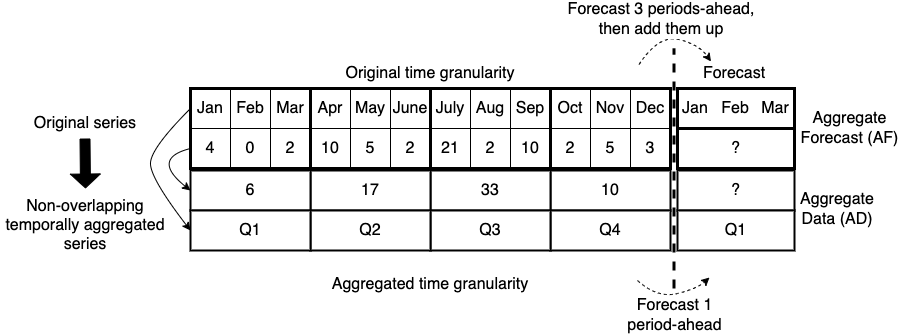
\includegraphics[width=0.9\linewidth]{img/300dpi/nota} \caption{Aggregate forecast vs. aggregate data approaches. Assuming a montly time series is available and a forecast over one quarter (aggregation level =m3 months) is required. We first generate forecast for 3 periods ahead and then sum them up to create forecast over the quarter (Forecast by AF approach). Then, we create the temporally aggregated series bu diviging the original series into the block of 3 periods. Next, we forecast for 1 period ahead (Forecast by AD approach).}\label{fig:example_oanoa}
\end{figure}

For the later, we often use the non-overlapping temporal aggregation
(NOTA) approach. Using this approach, the original series is divided
into a consecutive non-overlapping bucket of time, starting from the
most recent period backward. The size of the bucket is equal to the
number of time periods required in forecasting, which is referred to
aggregation level, \(m\). The aggregated series is then created by
summing up the values inside each bucket. The number of aggregate
observations is \([N/m]\), where \(N\) is the number of periods, and the
\([x]\) operator returns the integer part of \(x\) (Rostami-Tabar et
al., 2019). We should also note that non-overlapping temporal
aggregation

There are some studies that investigate this question when considering
forecasting at one single level of aggregation Kourentzes et al. (2017)
or forecast combinations using multiple temporal aggregation levels
(Kourentzes et al., 2014) or temporal hierarchies (Athanasopoulos et
al., 2017). These approaches have been applied Petropoulos and
Kourentzes (2014) in both intermittent demand (Nikolopoulos, 2021) and
fast-moving demand contexts (Athanasopoulos et al., 2017).

The overall conclusion is that both aggregate forecast and aggregate
data approaches may outperform each other. Their performance may depend
on the presence of the autocorrelation in the original series,
aggregation level, forecast horizon and the employed forecasting method
(see, e.g., Boylan and Babai (2016), Rostami-Tabar et al. (2021),
Rostami-Tabar et al. (2014) Nikolopoulos et al. (2011)). This study only
applies to the case of a single level of aggregation, we can extend this
study to examine the case of using multiple level of aggregation and
hierarchies in the future.

Despite recent development in this area, there is still a lack of rules
and indications on which approach should be used on each time series. In
particular, given the features of the time sires, there is no solution
of which strategy should be recommended to forecasters. This is the
first study that explores the association between time series features
and model performance in the context of forecasting by temporal
aggregation (TA). The need for such a research has also been emphasised
by Babai et al. (2021) in a review article. This paper aims to shed
lights on how the performance of temporal aggregation approaches
(i.e.~both AF and AD) is associated with time series features.

This study employs 48,000 time series from the monthly M4-competition
dataset to assess empirically the performance of each approach and then
examine the association between the original time series features and
the forecasting performance evaluation using machine learning models. We
then describe how non-overlapping temporal aggregation changes the
features of time series, going from a high granularity level
(e.g.~monthly) to a low granularity (e.g.~annual). Next, we discover
which features are critical in predicting accurately the performance of
each approaches, followed by an interpretation of features associated
with the performance of AD or AF approaches. This will help us to
provide recommendations to forecasters and decision makers on which
approach to use.

The research objectives are as following:

\begin{enumerate}
\def\labelenumi{\arabic{enumi}.}
\tightlist
\item
  We measure 42 features of the time series at the original level and at
  various levels of aggregation. We reveal how TA changes the time
  series features;
\item
  We examine the forecast accuracy performance of AD and AF;
\item
  We build a machine learning model using feature engineering to predict
  accurately the performance of each approach;
\item
  We examine the association between time series features and the
  forecasting performance;
\item
  We determine for which type of time series features, each forecasting
  strategy might be preferable;
\end{enumerate}

The rest of the paper is organised as follows: section \ref{lit}
provides a brief overview of the use of temporal aggregation in time
series forecasting. Section \ref{framework} describes the empirical
experiment design, forecasting approaches, method and forecast accuracy
metrics. model and notations. Section \{tsfeature\} describes time
series features and presents the time series features for monthly M4
competition datase, followed by analysing how non-overlapping temporal
aggregation affects time series features. We then examine the
forecasting performance of AD and AF approaches. Section \ref{ml}
presents machine learning algorithms and their performance on accurately
classifying the performance of AD and Af for a given time series and its
features. Section \ref{res} presents the important features and their
connection with the performance of temporal aggregation approaches.
Section \ref{con} provides concluding remarks and an agenda for future
research.

\hypertarget{lit}{%
\section{Research background}\label{lit}}

In practice, a time series is generally stored at a single level of time
granularity. When a time series is available at a higher granularity
level (e.g.~hourly, monthly), it is often expected to generate a
forecast at lower granularity (e.g.~daily, annual). Therefore, a
forecast of the total value over a number of time periods ahead
(i.e.~lead-time or aggregation level) is required (Mohammadipour and
Boylan, 2012). In these situations, an obvious option, that is often
recommended in practice (Goodwin, 2018), would be to first transform the
higher granularity time series into the lower granularity that matches
the forecast requirement, and then produce forecasts. The transformation
is generally performed using non-overlapping temporal aggregation.

Another approach is to aggregate forecast rather than data. In that
case, we first produce forecasts using the higher granular time series
for the forecast horizon (i.e.~multiple periods ahead) and then
aggregate them.

The application of NOTA approach in time series forecasting has been
initially studied in the econometric literature. They evaluated how NOTA
may change the structure of Autoregressive Integrated Moving Average
(ARIMA) processes (Rossana and Seater, 1995; Wei, 1978). This literature
is in favor of aggregated data using NOTA. They show that this approach
leads to accuracy gains under the assumption of ARIMA process and using
an optimal Conditional mean forecast.

Rostami-Tabar et al. (2013) and Rostami-Tabar et al. (2014) further
explored analytically the effect of NOTA on forecasting performance at
both aggregated forecast horizon ( lead time) and the disaggregated
level using Mean Squared Error (MSE). They assume that Single
Exponential Smoothing (SES) forecasting method is applied to an
ARIMA(1,1) time series. The determine the conditions under which
aggregate data outperforms the aggregate forecast approach. They show
that the superiority of each approach depends on the process parameters
that are affecting time series features, parameters of the forecasting
method, and aggregation levels. They conclude that NOA performs better
when autocorrelation is not highly positive. In contrast, they show that
high positive autocorrelation as one of the key features of time series,
favourites AF approach. Rostami-Tabar et al. (2019) evaluated the impact
of NOTA on forecasting demand and orders in a supply chain. They assume
that the demand time series follows an ARMA(1,1), the stock policy is
order-up-to-level and optimal forecasting is used to produce forecasts.
They showed that although the NOTA does not lead to an accuracy
improvement in terms of MSE at the retailer's level, however it can lead
to MSE reduction at the manufacturer level and a reduction of the
bullwhip effect..

Mohammadipour and Boylan (2012) also assessed analytically the effect of
temporal aggregation when the time series process is integer
autoregressive moving average, INARMA(\(p,q\)), processes. The
demonstrated that aggregate data leads to lower MSE compared to
aggregate forecast approach when the value of the autoregressive
parameter is high. They found that for short horizons and smaller values
the series process with small autoregressive and moving average
parameters and short length of forecast horizon.

The potential forecasting benefit of TA was investigated by Willemain et
al. (1994) and Nikolopoulos et al. (2011) in the context of intermittent
time series. Willemain et al. (1994) empirically compared the forecast
accuracy improvement of AF and AD approaches. They showed that
aggregating time series can lead to more accurate forecasts.
Nikolopoulos et al. (2011) show that an NOTA approach may offer
considerable improvements in terms of forecast accuracy. Further studies
(Babai et al., 2012; Kourentzes et al., 2014; Petropoulos and
Kourentzes, 2015; Spithourakis et al., 2011) confirmed empirically the
forecast and stock control improvement resulted from NOTA. These studies
covered both intermittent and fast moving time series.

Athanasopoulos et al. (2011) investigated the benefits of aggregate
forecast versus aggregate data in an empirical study consisting of 366
monthly series. Various forecasting methods including state space models
for exponential smoothing (ETS) and ARIMA, and the Theta are considered.
Their findings are in favor of aggregating forecast. They found that
aggregating forecast from either monthly or quarterly to yearly leads to
more forecast accuracy improvements than yearly forecasts generated from
the NOTA yearly series. Using time series of order and point-of-sale in
a retail supply chain, Jin et al. (2015) assessed the benefits of NOTA
for forecast accuracy. They found that NOTA leads to more accurate
forecasts when the autocorrelation of time series is not highly
positive. In a study where a high frequency time series is used, Luna
and Ballini (2011) showed that in daiy forecast of cash withdrawals,
NOTA results in similar or better forecast than using hourly series.

Some studies have investigated the benefits of producing forecasts using
multiple time series resulted from NOTA approach, corresponding to
multiple levels of aggregation. Forecasts are generated at each level
and then combined to obtain the required forecast. Kourentzes et al.
(2014) recommended using multiple levels of aggregation and combining
the separate forecasts (MAPA). Multiple studies in intermittent time
series forecasting, promotional modeling and inventory management
highlighted the gain of using multiple TA levels Barrow and Kourentzes
(2016). Athanasopoulos et al. (2017) proposed Temporal Hierarchies
Forecasting (THieF), which creates multiple temporally aggregated series
using NOTA, generate forecasts and then reconciles them to obtain the
required forecast.

Collopy and Armstrong (1992) developed a rule-based system containing 99
rules to produce forecasts based on the features of the data.

developed a rule-based system containing 99 rules to produce forecasts
based on the features of the data. Adya et al.~(2001) identied
time-series features automatically for rule-based forecasting.
Petropoulos et al.~(2014) explored the factors that aect forecasting
accuracy in the eld of demand forecasting, and proposed related
selection protocols. Kang et al.~(2017) used Principal Component
Analysis (PCA) to visualize the forecasting algorithm performance in the
time series instance spaces and had a better understanding of their
relative performance. Finally, Talagala et al.~(2018) used a decision
tree to select the best forecasting method based on 42 manual features.

Another approach that also uses data manipulation to extract additional
information is (non-overlapping) temporal aggregation (Nikolopoulos et
al., 2011).

M4 data set in the M4comp2018 R package (Montero-Manso et al., 2018).

Although all approaches including AF, AD and using multiple TA levels
have demonstrated forecasting gain, arguably none of them are suitable
to be used in every situation. Almost all studies in the literature
report an overall accuracy (e.g.~average) rather than accuracy at the
time series level. We argue that some time series features may favorite
using a particular approach over other. However there is no study in the
literature that investigates the potential association between time
series features and approach performance. This study will cover this gap
by considering forecasts resulted from AF and AD approaches.

\hypertarget{framework}{%
\section{Experiment framework}\label{framework}}

In this section, we describe the design of the empirical experiment used
in this study. We first present the study framework, then introduce the
forecasting approaches and method, followed by showing the forecasting
error metrics.

Figure \ref{fig:expdes} illustrates the framework of the experimental
design performed in this study. The framework consists of several steps
which are described as following. For any time series, we complete the
following steps:

\begin{enumerate}
\def\labelenumi{\arabic{enumi}.}
\item
  The original time series is transformed into temporally aggregated
  series for a given aggregation level, \(m\);
\item
  A set of features is extracted for the original and aggregated time
  series;
\item
  A forecasting method (i.e.~ETS) is applied to the original series to
  generate forecast for \(m\) periods ahead;
\item
  Forecasts per each period are added up to obtain the forecast over the
  aggregated horizon (forecasts from AF);
\item
  Forecasts are generated for temporally aggregated series (forecasts
  from AD);
\item
  Forecast accuracy is calculated for each series;
\item
  A databas consisting of time series features and the performance of
  the AF and AD approaches is constructed. Time series features are used
  as an input (predictors) and the winning approach (labeled as AF or AD
  based on the minimum error metric) creates the response variable;
\item
  Several machine learning (ML) models are built to accurately predict
  the superiority of AF/AD approaches using the data created in step 7.
  These models include: 1) Logistic regression (LR), 2) Linear
  discriminant analysis (LDA), 3) Quadratic discriminant analysis (QDA),
  4) K-Nearest Neighbors (KNN), 5) Lasso, 6) Generalised Additive Model
  (GAM), 7) Boosting, 8) Support Vector Machine (SVM) and 9) Random
  Forest (RF). Rehears are referred to James et al. (2021) for a detail
  description of these approaches. Given the outperformance of the
  random forest among among all ML models used in this study, we will
  describe it in more details in section \ref{ml}.
\end{enumerate}

The ML model can also help us to identify the most important time series
features that lead to the outperformance of RF. Moreover, it can also
reveal how time series features are connected to the performance of
AD/AF.

Due to the page restriction, details regarding the initial set up,
method of optimization, cost function, etc of these algorithms; are
available by request from the authors. The experiment has been conducted
in R software, and the authors are happy to share the code for
reproducibility upon request.

\begin{figure}[H]

{\centering 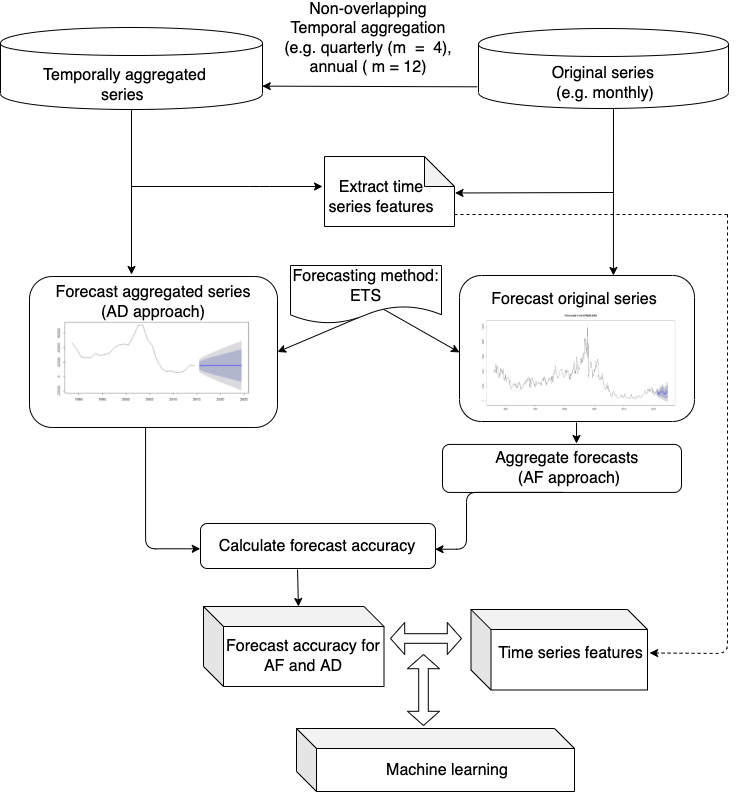
\includegraphics[width=0.7\linewidth]{img/300dpi/experiment_design} 

}

\caption{Design of the experiment framework}\label{fig:expdes}
\end{figure}

\hypertarget{forecasting-approaches}{%
\subsection{Forecasting approaches}\label{forecasting-approaches}}

We consider two different approaches to produce the forecast horizon
aggregation. Given that the original time granularity is monthly, we aim
at generating forecasts for various aggregation levels that corresponds
to 2-monthly (m = 2), quarterly (m = 3), 4-monthly (m = 4), semi-annual
(m = 6) and annual (m = 12) time granularity.

The first approach is to aggregate forecasts (AF). This approach first
involves creating the base forecasts for \(m\) periods ahead. These
forecasts are then aggregated, because forecasting at the aggregation
horizon level is of interest. The main advantage of AF is that there is
no loss of information from the data because initial base forecasts are
generated at the lowest disaggregated level. AF approach can capture the
dynamics of the high frequency series, however they may be noisy and
difficult to model. In the case of stationary time series, the AF
approach may produce a more accurate forecast when the autocorrelation
of the underlying demand series is highly positive (Rostami-Tabar et
al., 2014). Conversely, there is an absence of researches in the case of
non-stationary time series. Therefore, this research is dealing with
both stationairy and non-stationary time series and provides insight
into the perplexity of interactions between different factors that
influence on AF approach.

The second approach is to aggregate data (AD). This approach consists of
applying the non-overlapping temporal aggregation approach to the
original series, using the time granularity level for which the
forecasting is needed. Following that the process of forecasting the
temporally aggregated series for one atep ahead is performed. Benefits
of AD can be seen in the reduction of the noise in the data, as well as
in revelling the more smooth patterns that exist in the series. The NOTA
of the series usually sheds light on the key time series features, which
are more notable and clearer as we perform the aggregation to the lower
granularity levels (e.g.~quarterly, annual).

\hypertarget{forecasting-method}{%
\subsection{Forecasting method}\label{forecasting-method}}

The exponential smoothing state space (ETS) models (Hyndman and
Athanasopoulos, 2021) are used to produce out of sample forecasts,
although our experiment design is model agnostic and could be expanded
to any other forecasting model. ETS can capture trend, seasonality and
error components in a time series through various forms such as
additive, multiplicative or mixed. ETS accounts for 18 different
exponential smoothing models. The automatic exponential smoothing model
is used using \emph{ets()} function in the forecast package (Hyndman and
Khandakar, 2008) in R to produce forecasts for the original and
aggregated time series. For each series, \emph{ets()} identifies the
most accurate model using the corrected Akaike's Information Criterion
(AICc). Using an automatic forecasting method such as ETS is suitable
for this study, as we can assume that the best model is selected for
each series and this may help to separate the effect of the applied
forecasting method from TA approaches (i.e.~AF and AD).

\hypertarget{errormetric}{%
\subsection{Forecast accuracy measures}\label{errormetric}}

In this experiment, forecast accuracy evaluation is required two
different stages.

We first use an error metric (e.g.~Root Mean Squared Scaled Error) to
quantify the forecast accuracy of AF and AD in generating time series
forecast over leadtime for each time series and ETS method. We consider
the in-sample and the out-of-sample sets in monthly M4 competition time
series. We apply the ETS method to each series in the in-sample dataset
and keep their forecast for the out-of-sample using time series cross
validation with re-estimation. The forecast horizon for the original
time series equals \(m\), the aggregation level, and the horizon for
non-overlapping aggregated series is one. We then compute the forecast
errors over the test period of each time series. To evaluate the
forecast accuracy and bias, several measures including Root Mean Squared
Error (RMSE), Mean Absolute Error (MAE) and Mean Error (ME), Mean
Absolute Percentage Error (MAPE), Mean Absolute Scaled Error (MASE) and
Root Mean Squared Scaled Error (RMSSE) are used. Due to the space
restriction, we only present results of the RMSSE. Forecast accuracy
results for other error metrics are available by request. RMSSE is given
by:

\[ \text{RMSSE} = \sqrt{\text{mean}(q_{j}^2)},\] where

\[q^2_{j} = \frac{\displaystyle e^2_{j}}
    {\displaystyle\frac{1}{T-m}\sum_{t=m+1}^T (y_{t}-y_{t-m})^2},\]

Second, we need to report how accurately a classification model predicts
the outcome (i.e.~the most accurate approach labeled as AF and AD), when
presented with a set of time series features at the original series. To
that end, we report several statistical measures including
misclassification error, F-statistics and area under the curve (AUC).

The misclassification error is calculated as following:

\[Misclassification_{error} = 100\% \times \left( 1-\frac{(t_p+t_n)}{N}\right),\]

F statistic is defined as:

\[F_{statistics} = 2 \times 100\% \times \left(\frac{(tp/(tp+fp) \times tp/(tp+fn))}{(tp/(tp+fp)+tp/(tp+fn)}\right),\]

Where \(t_p\) is true positive, \(t_n\) is true negative, \(f_p\) is
false positive and \(f_n\) is false negative.

The false positive rate represents the fraction of test cases in which
AD was incorrectly classified as a right model to use, while in reality
the AF was the correct one. Similarly, the false negative rate
represents the fraction of test cases in which AF was incorrectly
classified as a right model to use, while AD was the correct one.

The area under the curve (AUC) represents the surface that is
encompassed under the receiver operating characteristics (ROC) curve
{[}James et al. (2021). The larger the area under the ROC curves the
better the classifier. The maximum value of AUC is 1, which would be
considered a perfect classifier. Conversely, the classifier that
performs no better than chance will have an AUC of 0.5 and would be
considered as a very poor one.

In addition to the statistical measures discussed above, we also perform
the utility evaluation of different models. The utility metric
approximates the costs and benefit of wrong and correct classification.
For that purpose, average RMSSE error is used as a utility metric.

To assess the prediction accuracy of ML models, we split the data
created in the step 7 of \ref{framework} into a training and a test set.
To that end, we randomly divided the data on train and test set in a
70/30 \% split. The train data (33600 cases) is used for training
different algorithms, while the test data (14400 cases) is used for
evaluating the model's performance.

\hypertarget{tsfeature}{%
\section{Time series data, features and temporal aggregation
performance}\label{tsfeature}}

In this section, we first introduce the time series features extracted
for each time series. Following that, we illustrates these features for
the monthly M4 competition dataset,. The, we describe how
non-overlapping temporal aggregation affects these features. Finally, we
discuss the forecasting performance of AD and AF applied on monthly M4
dataset.

\hypertarget{time-series-features}{%
\subsection{Time series features}\label{time-series-features}}

Table \ref{tab:summaryfeature} presents the description of 41 features
used in this study. For each time series (original or aggregated), we
compute a set of measures from the training data. These features are
also described in detail by Wang et al. (2009) and Hyndman et al. (2015)
and Hyndman and Athanasopoulos (2021).

\begin{table}[!h]

\caption{\label{tab:summaryfeature}Time series features considered in this study and their descriptions}
\centering
\resizebox{\linewidth}{!}{
\fontsize{11}{13}\selectfont
\begin{tabular}[t]{ll}
\toprule
Feature & Description\\
\midrule
mean & mean\\
var & Varince\\
cv & Coeifficnet of variation\\
trend & Strength of trend, a value close to 1 indicate highly trended series\\
seasonal\_strength & strength of seasonality, a value close to 1 indicate highly seaonal series\\
entropy & Measure of how easy the series is to forecast. Entropy close to 0 shows a series  is easy to forecast\\
lumpiness & Lumpiness is the variance of the variances of  tiled (non-overlapping) windows\\
flat\_spots & Number of sections of the data where the series is relatively unchanging\\
crossing\_points & Number of times a time series crosses the median\\
nonlinearity & Extent of nonlinearity, if values around 0  series is linear. Large values shows nonlinearity\\
stability & Stability is the variance of the means of  tiled (non-overlapping) windows\\
hurst & Hurst coefficient of a time series which is a measure of ong memory\\
spike & Prevalence of spikes in the remainder component  of the STL decomposition\\
linearity & Linearity of the trend component of the STL decomposition\\
curvature & Curvature of the trend component of the STL decompositio\\
peak & Timing of the peaks\\
trough & Timing of the troughs\\
x\_acf1 & First autocorrelation coefficient\\
x\_acf10 & Sum of squares of the first ten autocorrelation coefficients\\
diff1\_acf1 & First autocorrelation coefficient from the differenced series\\
diff1\_acf10 & Sum of squares of the first ten autocorrelation coefficients from the differenced series\\
diff2\_acf1 & First autocorrelation coefficient from the twice differenced data\\
diff2\_acf10 & Sum of squares of the first ten autocorrelation coefficients from the twice differenced series\\
seas\_acf1 & Autocorrelation coefficient at the first seasonal lag\\
x\_pacf5 & Sum of squares of the first 5 partial autocorrelation coefficients\\
diff1x\_pacf5 & Sum of squares of the first 5 partial autocorrelation coefficients of differenced series\\
diff2x\_pacf5 & Sum of squares of the first 5 partial autocorrelation coefficients of second-order differenced\\
seas\_pacf & Partial autocorrelation coefficient at the first seasonal lag\\
unitroot\_kpss & Kwiatkowski-Phillips-Schmidt-Shin (KPSS) test\\
unitroot\_pp & Phillips-Perron statistic for testing if a series is non-stationary\\
arch\_acf & Sum of squares of the first 12 autocorrelations of squared series\\
garch\_acf & Sum of squares of the first 12 autocorrelations of residuals, after fitting an GARCH(1,1)\\
arch\_r2 & R2 value of an AR model applied to the squared series\\
garch\_r2 & R2 value of an AR model applied to  residuals, after fitting an GARCH(1,1)\\
ARCH.LM & Statistic based on the Lagrange Multiplier (LM) test  for autoregressive conditional heteroscedasticity (ARCH)\\
e\_acf1 & First autocorrelation coefficient of the remainder series\\
e\_acf10 & Sum of squares of the first ten autocorrelation coefficients of the remainder series\\
max\_level\_shift & Largest mean shift between two consecutive sliding windows of the time series\\
time\_level\_shift & Timing index of the largest mean shift between two consecutive sliding windows of the time series\\
max\_var\_shift & Largest variance shift between two consecutive sliding windows of the time series\\
time\_var\_shift & Timing index of the largest variance shift between two consecutive sliding windows of the time series\\
\bottomrule
\end{tabular}}
\end{table}

\hypertarget{mtsmeasure}{%
\subsection{Time series features of monthly M4 data}\label{mtsmeasure}}

We use the monthly M4 competition time series to empirically examine the
performance of AD and AF and investigate the connection between their
performance and time series features. The monthly M4 data contains
48,000 time series. The dataset comes from the Economic, Finance,
Demographics and Industry areas, while also including data from Tourism,
Trade, Labor and Wage, Real Estate, Transportation, Natural Resources
and the Environment (Makridakis, 2018). The monthly data is the most
important data for the business applications (Spiliotis et al., 2020)
and therefore the largest class in M4, containing almost half of the
data (48000 time series).

For each time series in the monthly M4 dataset, we extract 41 features
as described in Table \ref{tab:summaryfeature} using \emph{tsfeatue()}
function in the forecast package in R (Hyndman and Khandakar, 2008).
Figure \ref{fig:feature1} and \ref{fig:feature2} illustrates the
corresponding distribution of each feature. Y-axis shows the frequency
in terms of the number of time series, and X-axis indicates the range of
values extracted for each feature. This figure shows that the monthly M4
dataset covers a wide range of time series features, which makes it a
suitable data for this research problem. Additionally, we include the
origin of the time series M4 competiton data, i.e.~Economic, Finance,
Demographics and Industry, as the 42nd feature.

The spectral entropy plot indicates that there is a range of time series
from easy (less noise, more systematic information) to hard (more noise,
less systematic information) to forecast. Coefficient of Variation is
also skewed to the right and indicates less variability for the majority
of series.

The trend peaks near one and is skewed to the right indicating the
strong presence of the trend in this dataset. We also observe that the
nonlinearity feature peaks near zero and it is skewed to the right,
which indicates the lack of nonlinearity in the time series. The
autocorrelation lag1 and seasonal autocorrelation lag1 is skewed to the
left, and is highly positive for many time series. We also measure the
seasonal autocorrelation lag1 which is highly positive and : seasonal
autocorrelation lag1 is high, and The lumpiness is extremely low for
almost all time series and stability has a range from low to high
values. We also measure seasonal partial autocorrelation and the
strength of seasonality, both indicate a lower strength of seasonality.
We also measure the stationaity(non-stattioanirity) of series using both
unitroot\_pp and unitroot\_kpss statistics. They indicate a strong
presence of staitonairy time series. Curvature shows a sharp
distribution centered around zero meaning most series do not have
stochastic or chaotic nature. In particular, time series of stochastic
nature are associated --\textgreater{} with curves displaying positive
curvature in a neighborhood of their initial points, whereas curves
related to chaotic phenomena have a negative curvature

Hurst has a left skewed distribution with almost all series with a
values very close to one indicating the presence of the long memory for
series, which is related to the autocorrelations. max\_level\_shift is
centered around one and has a range of values between 0 and 3.

ARCH.LM (A time series exhibiting conditional heteroscedasticity---or
autocorrelation in the squared series---is said to have autoregressive
conditional heteroscedastic (ARCH) effects.) (if ARCH.LM is close to 1,
means there is ARCH effect?

The distribution of the e\_acf10 values is skewed to right and the plot
shows that for most of the time series e\_acf10 is close to zero, which
means the leftover from trend and seasonality seems to be random.

Readers can refer to the figure for the rest of features of monthly M4
time series.

\begin{figure}[H]

{\centering 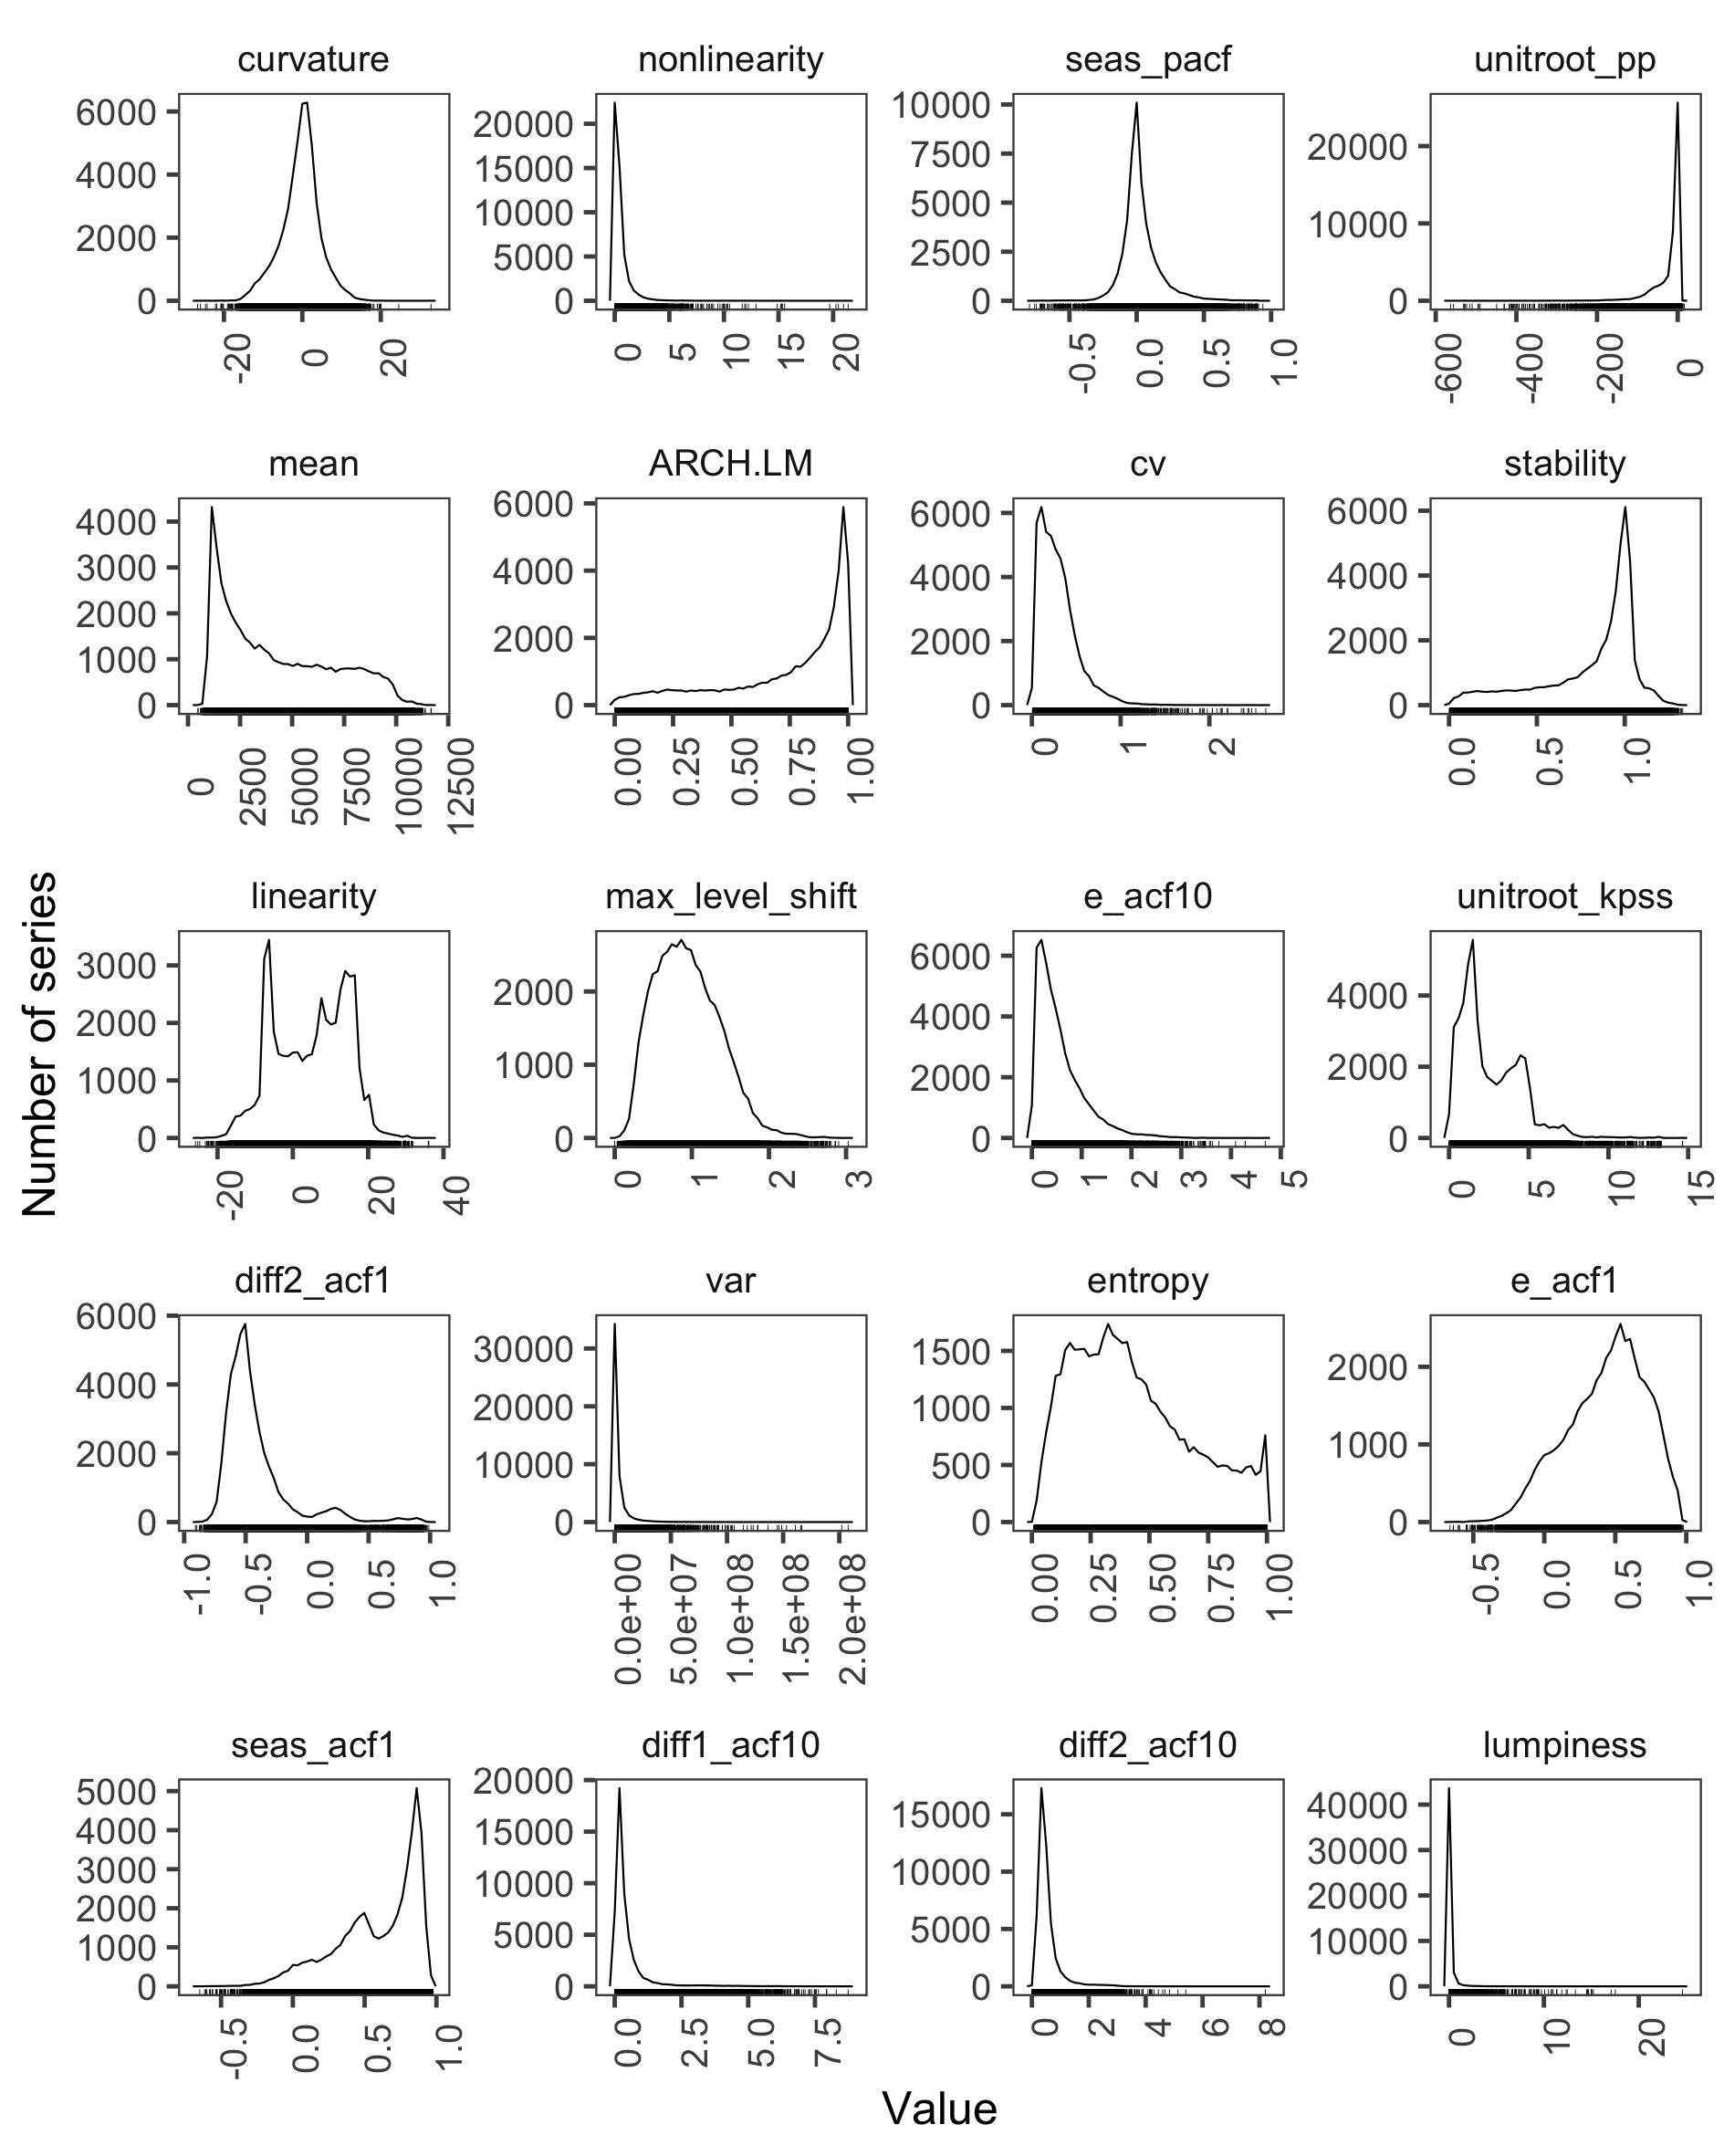
\includegraphics[width=0.7\linewidth]{img/300dpi/featurets1} 

}

\caption{Features of monthly time series from M4 competition dataset}\label{fig:feature1}
\end{figure}

\begin{figure}[H]

{\centering 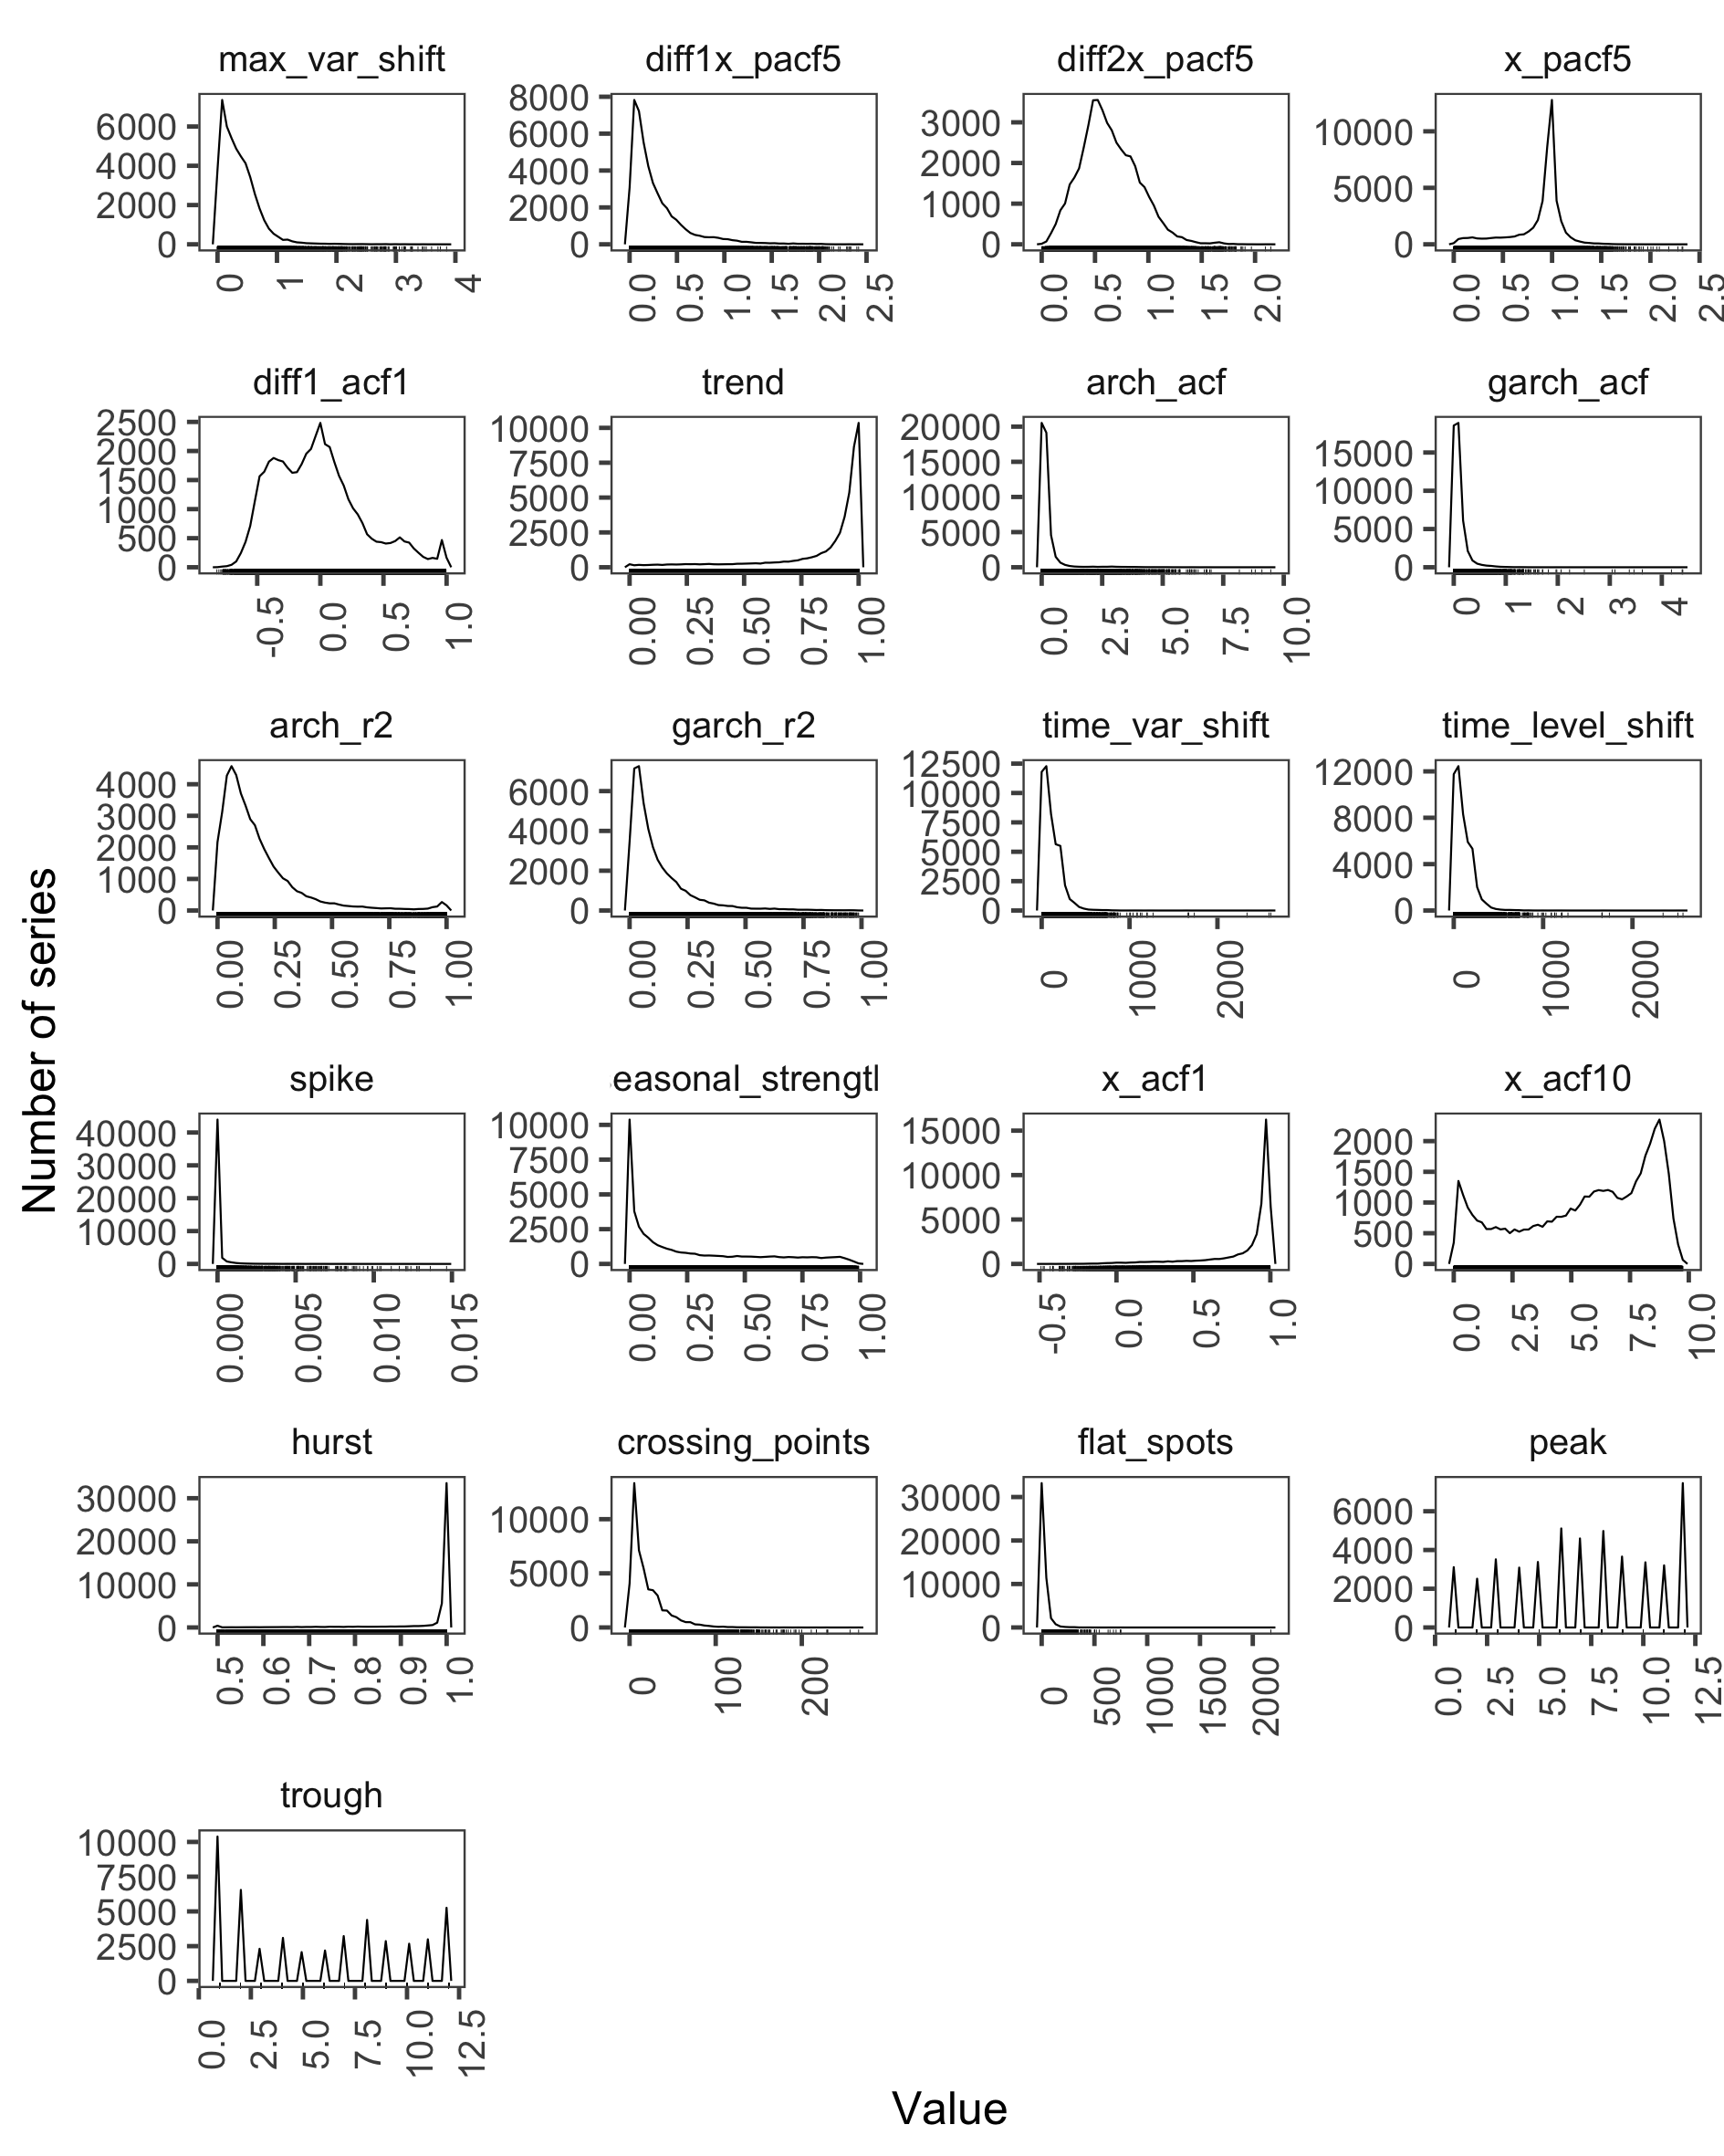
\includegraphics[width=0.7\linewidth]{img/300dpi/featurets2} 

}

\caption{Features of monthly time series from M4 competition dataset (continue)}\label{fig:feature2}
\end{figure}

\hypertarget{taeffect}{%
\subsection{Effect of temporal aggregation on time series
features}\label{taeffect}}

In addition to extract the futures of the monthly time series, we also
compute features after transforming the time series to bi-monthly,
quarterly, 4-monthly, semi-annual and annual granularity. We use these
features to demonstrate how non-overlapping temporal aggregation may
change time series features. To highlight the effect of NOTA, we first
started by plotting the distribution of features at each level, however
the difference between distributions was not revealing because features
have log-tail distributions. Instead, we categorise features of the
original series to into four categories using quantiles:

\begin{itemize}
\tightlist
\item
  If \(0 < feature \leqslant 0.25\), Category = Very low
\item
  If \(0.25 < feature \leqslant 0.5\), Category = Very low
\item
  If \(0.5 < feature \leqslant 0.75\), Category = Very low
\item
  If \(0.75 < feature \leqslant 1\), Category = Very low
\end{itemize}

We then calculate the mean of features for each category and each time
granularity to create the figures. The results have been demonstrated in
Figure \ref{fig:feature1} and \ref{fig:feature2}. They show how time
series features are changing from monthly to annual granularity for the
time series features. The results indicate that as the level of time
granularity increases from monthly to annual, some features become
weaker and may disappear, while others dominate the series. The effect
has been clearly indicated in Figure \ref{fig:feature1} and
\ref{fig:feature2}.

\begin{figure}[H]

{\centering 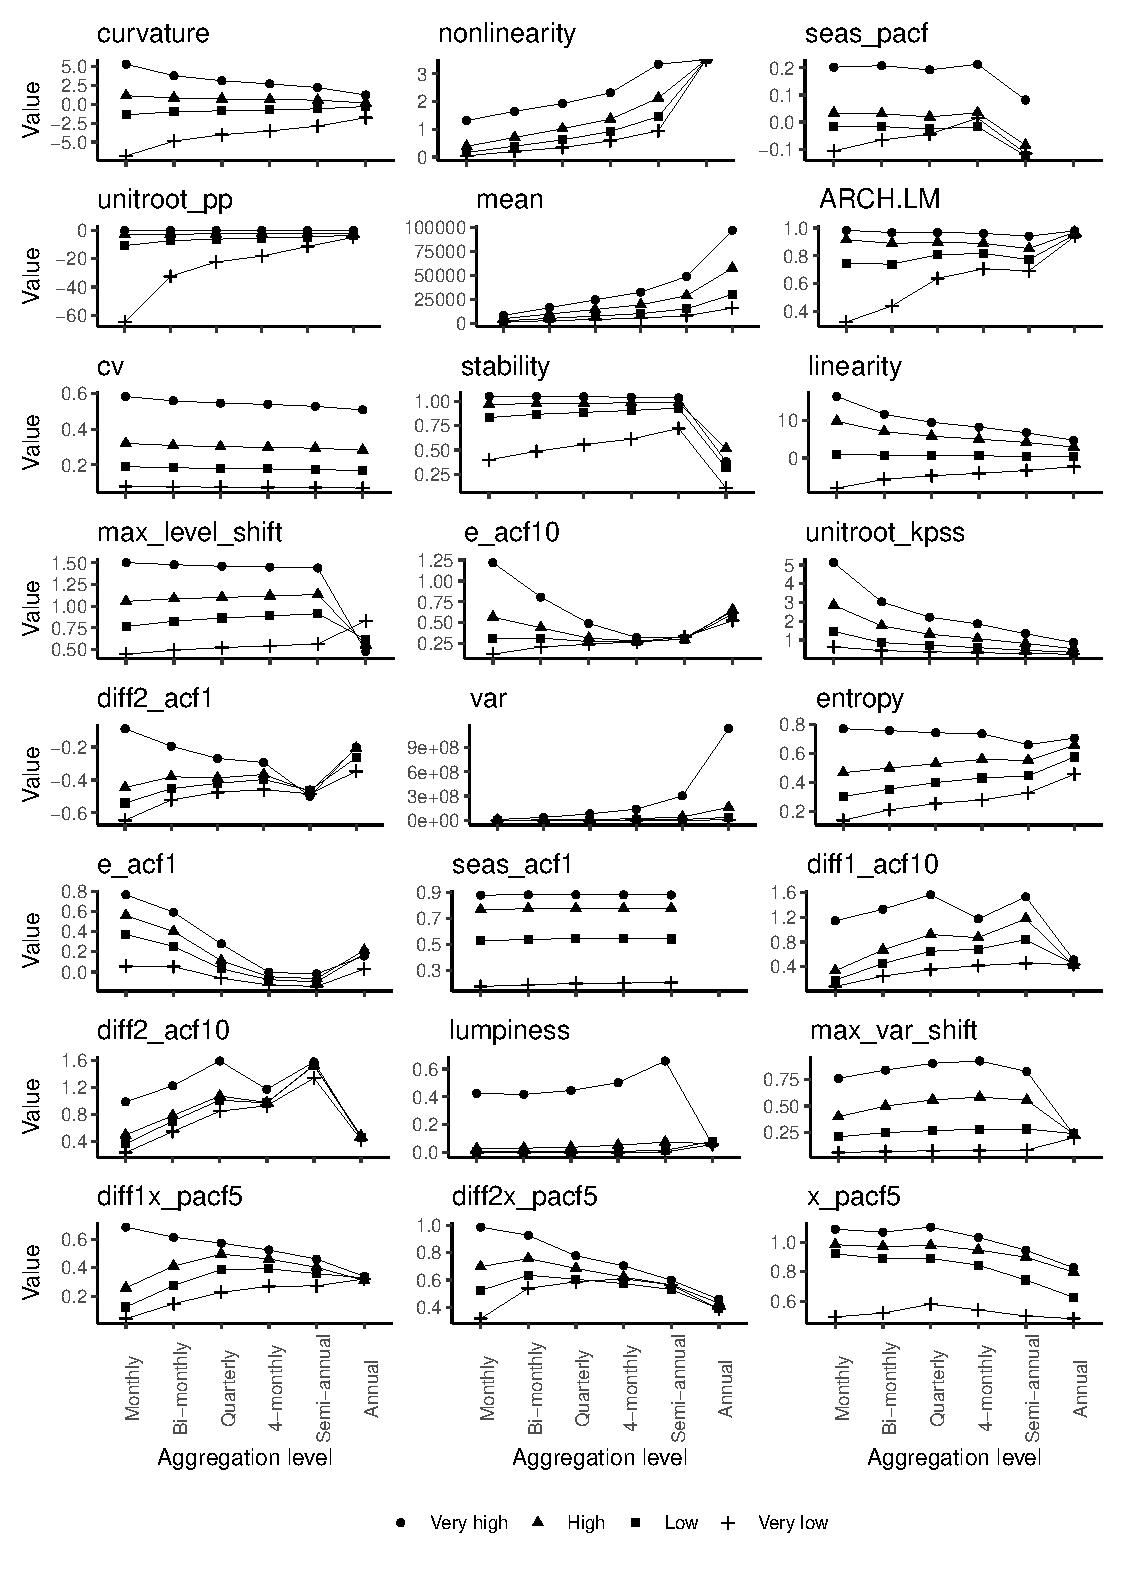
\includegraphics[width=0.7\linewidth]{img/mp_category_all1} 

}

\caption{The effect of non-overlapping temporal aggregation on monthly time series features of M4 competition dataset}\label{fig:featureagg1}
\end{figure}

We observe a decrease in curvature as we aggregate and it approaches
zero at annual level, while non-linearity increases with aggregation
indicating that series become more non-linear. Mean increases and
variance decreases, however the effect is higher for very high category.
We also observe that coefficient of variation decreases. Linearity is
pushed toward zero if it is high or low, meaning that series at annual
level losses its linearity feature. Both uniroot\_pp and unitroot\_kpss
become close to zero with increasing aggregation level, highlighting the
fact that series become more non-staitonairy if the monthly series if
staitonairy, other wise it remaoins almost the same. The measures
related to seasonality such as seasonal strength, autocorrelation lag1
and the sum of squared of the first 10 autocorrelation decreases. It is
interesting to observe that entropy increases with aggregation if it is
not very high at monthly level, meaning that series become difficult to
forecast. However we see a reduction in entropy if it is very high at
the monthly level. We also observe an increase for ARCH.HM especially if
it is very low at the monthly level. If it is very close to one, it
stays almost unchanged.

\begin{figure}[H]

{\centering 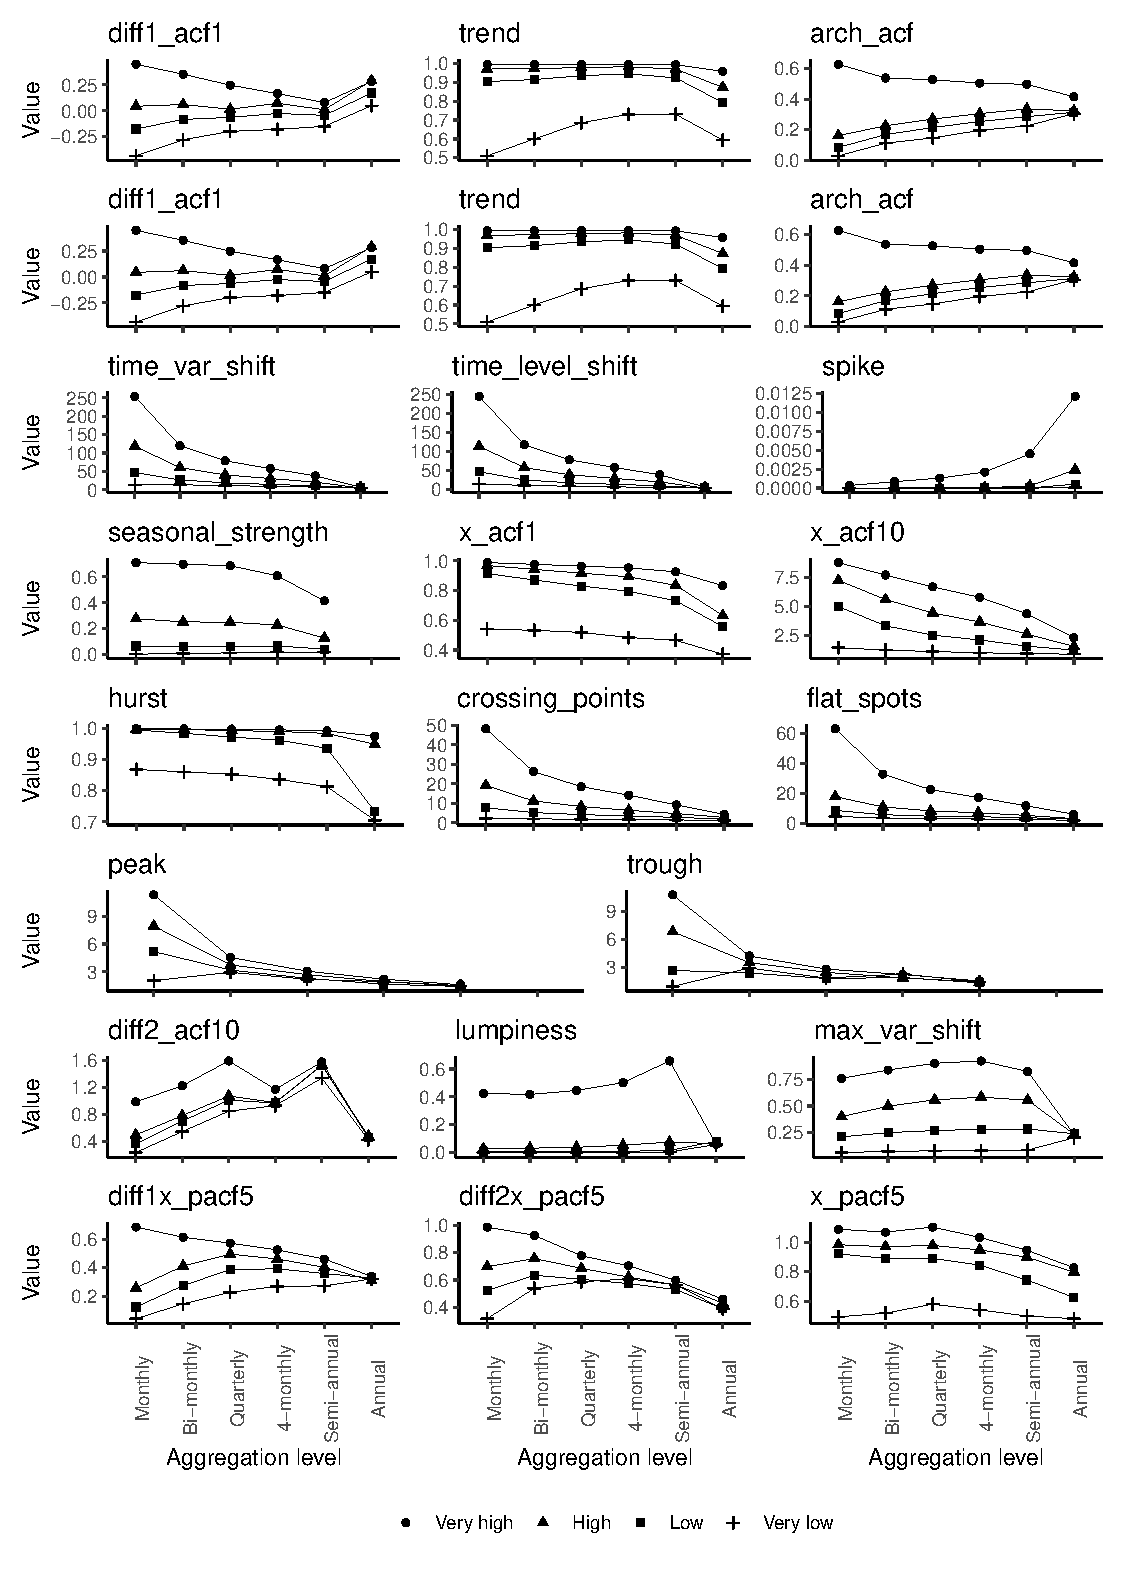
\includegraphics[width=0.7\linewidth]{img/mp_category_all2} 

}

\caption{The effect of non-overlapping temporal aggregation on monthly time series features of M4 competition dataset (continue)}\label{fig:featureagg2}
\end{figure}

We observe that the by approaching the annual level, some features
become unstable and showing chaotic behavior. We believe that this might
be due to the fact that seasonality in the annual level is not
calculated because the frequency equals. However, the seasonality index
might be used in calculating other features, hence the disorder of these
features at annual level.

\hypertarget{forecast-accuracy-evaluation-of-ad-and-af-approaches}{%
\subsection{Forecast accuracy evaluation of AD and AF
approaches}\label{forecast-accuracy-evaluation-of-ad-and-af-approaches}}

In this study, we aim at generating forecasts for a forecast horizon
aggregation /leadtime period using AF and AD approaches. While the
original time series temporal granularity is monthly, we require
forecasts to be produced at Bi-monthly (aggregation level = 2),
Quarterly (aggregation level = 3), 4-monthly (aggregation level = 4),
Semi-annual (aggregation level = 6) and annual (aggregation level = 12).

Figure @ref(fig:RMSSE) illustrates a Boxplot of RMSSE measure created
for all 48,000 series at various level of forecast granularity
requirement. Results demonstrate that both AF and AD approaches might
outperform each other for different time series. However, AF approach is
generating consistently more accurate forecasts through all aggregation
levels and the difference becomes more pronounced as aggregation level
increases. The difference is especially notable at the annual level.
From 48000 monthly time series, the AF approach was superior in 30147
cases (63\%) compared to 17853 cases (37\%) for AD when forecasting
annual time granularity. These results might be surprising regarding,
because most findings in the literature recommend using NOTA over
aggregate forecast and show improvements achieved on using temporal
aggregation as discussed in section @ref\{lit\}. However, we should note
that almost all of these studies report the overall accuracy
improvement, rather than the forecast accuracy at the series level. This
study shows that recommending AD to forecast over the forecast horizon
aggregation/leaddtime might not necessarily lead to more accurate
forecasts. Moreover, our results indicate that AF is a very competitive
forecasting strategy. This might be also due to the time series features
of the monthly time series discussed in section \ref{mtsmeasure}.

\begin{figure}[H]

{\centering 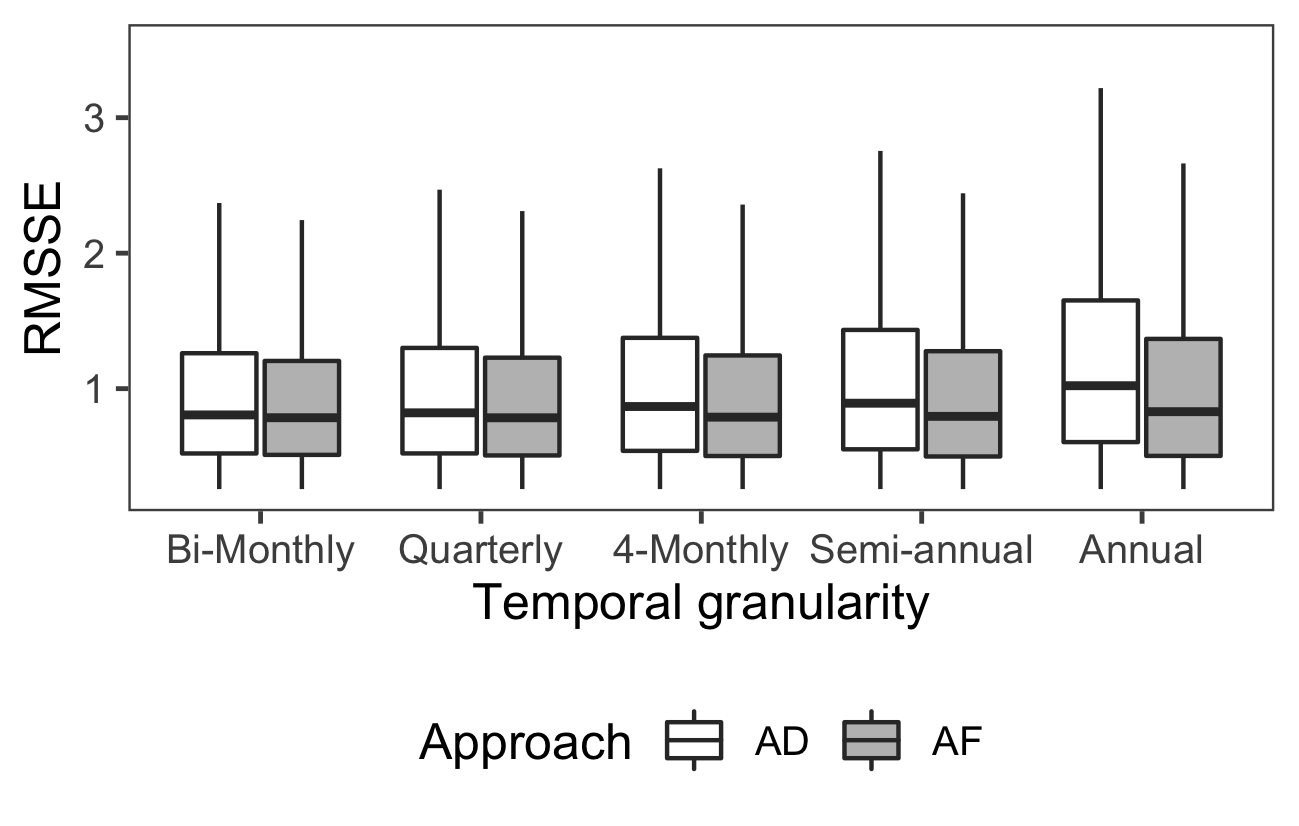
\includegraphics[width=0.7\linewidth]{img/300dpi/box_plot_rmsse} 

}

\caption{RMSSE errors through aggregation levels.}\label{fig:RMSSE}
\end{figure}

We have also conducted a statistical test using MCB (Multiple Comparison
with the Best method) (Koning et al., 2005) to assess the statistical
significance in the performance of AF and AD approaches.

From Figure @ref(fig:MCB), it is evident that there is a statistical
difference between forecasts generated from AF and AD. The forecasts
generated from AD approach are less accurate, while the strategy of
aggregating forecasts proves to be more accurate. The results were
cross-validated through multiple forecast horizons (h=12, 24 and 60) and
via several other error metrics as described in @ref(errormetric). The
main conclusions are almost perfectly aligned with already demonstrated
results in Figure \ref{fig:MCB}.

\begin{figure}[H]

{\centering 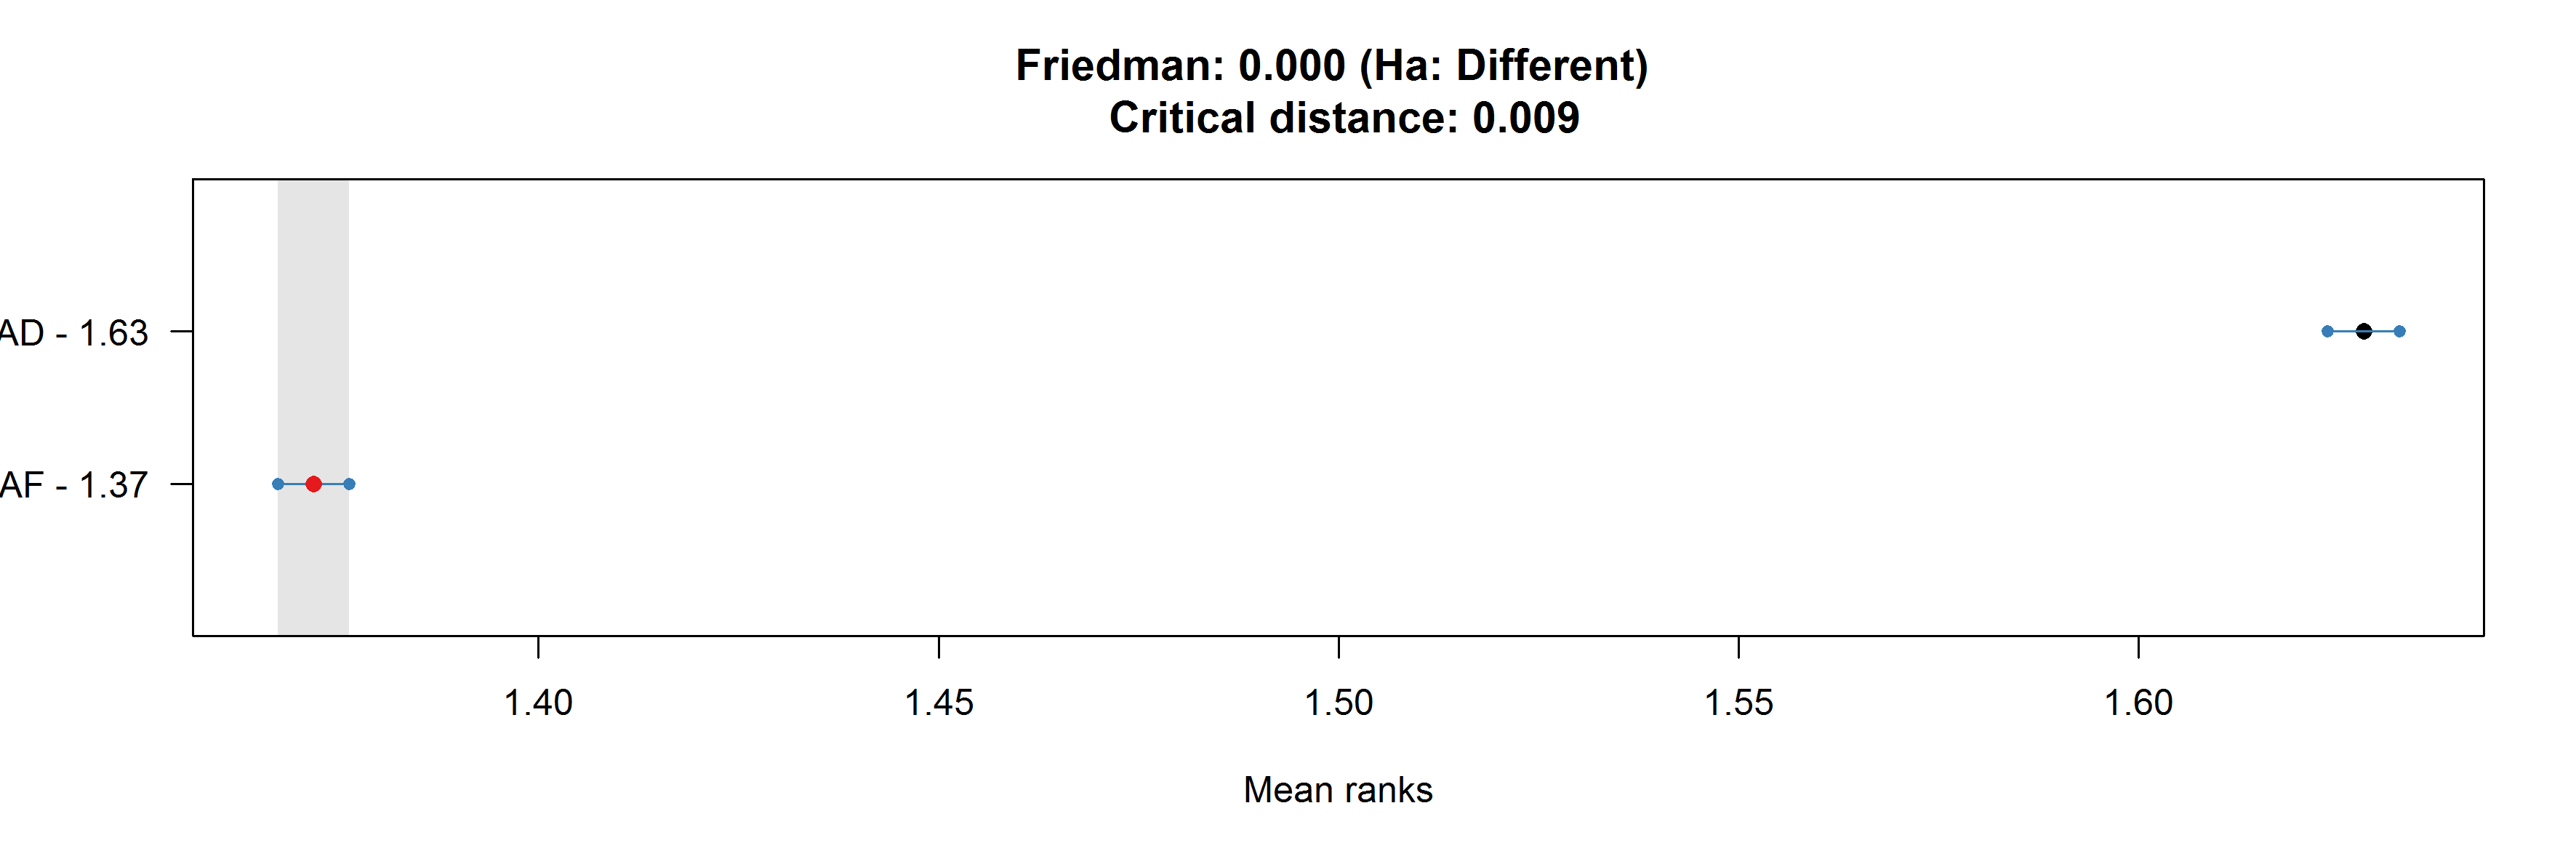
\includegraphics[width=1\linewidth]{img/300dpi/Fig_MCB} 

}

\caption{Performance of BU and DA models evaluated through MCB test. RMSSE errors are used for computing the ranks and a 95 percentile confidence level.}\label{fig:MCB}
\end{figure}

In Figure \ref{fig:RMSSE} we showed that both AF and AD have diverging
performance through different levels of aggregation. Moreover, Figure
\ref{fig:featureagg1} and \ref{fig:featureagg2} demonstrate the
evolution of the time series features through these levels. Therefore,
we argue that time series features can provide answers on why a
particular approach is favorable in different situations. We should note
that the results presented for the rest of paper are based on AF and AD
approaches to forecast annual aggregation level. There are multiple
reasons to support this: 1) we see the highest difference in the
performance at the annual level, ii) when the time series granularity is
monthly, it is often the case that forecast requirement time granularity
is annual, and iii) we investigated the analysis with other revels. In
the next section, we explore the association between time series
features and AF and AD performance and build machine learning models for
that purpose.

\hypertarget{ml}{%
\section{Machine learining models}\label{ml}}

In this section, we use machine learning models to shed lights on the
association between time series features and the performance of these
approaches. Using the time series features at monthly time granularity
and the RMSSE error metric generated for each approach (i.e.~AF and AD),
we build a machine learning algorithm to reveal relevant sets of
features affecting the performance of these approaches. The first step
in building such a model is to construct a dataset consisting of time
series features and model class labels for a given time series.
Therefore, we turn this problem into a classification supervised
learning, using features as predictors and the winning approach (i.e.~AD
or AF) as the response variable or outcome for each time series. We
discover, extract and present the details on which time series features
are the most influential on the accuracy of AF and AD approaches. In
addition to interpretability, the algorithm should be able to accurately
predict which model to use with a given set of the time series features
in the original time series. We should note that we have use the RMSSE
at the annual level given the pronounced difference in accuracy at that
level, however the conclusion should remain the same, if we use other
level of aggregations (i.e.~Semi-annual,4-monthly,Quarterly,bimonthly)
in the machine learning algorithms.

Figure \ref{fig:featuresmatrix} in the Appendix shows a grid of
scatterplots showing the bivariate interactions between various pairs of
features. Each point corresponds to one time series. The figure also
highlights the winning approach (i.e.~either AF or AD) when forecasting
for annual time granularity. The black dots represent the situations
where AD was more accurate, while yellow dots represent the opposite.
Given the number of features used in this study, it is unfeasible to
include the scatterplot matrix for all pairs of features. Figure
\ref{fig:featuresmatrix} shows only the pairs plot for 10 features.

\begin{figure}[H]

{\centering 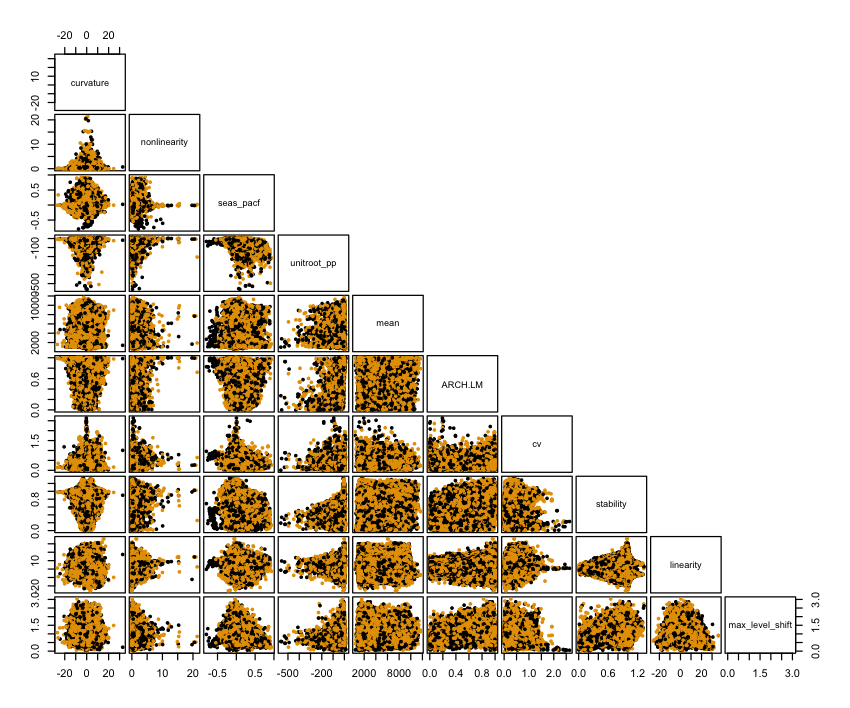
\includegraphics[width=1\linewidth]{img/300dpi/pair_plot} 

}

\caption{Time series features matrix. Each point indicates one single time series with a feature in x-axis and another at y-axis. The black and yellow colors show the outperformance of AD and AF, respectively.}\label{fig:featuresmatrix}
\end{figure}

Figure \ref{fig:featuresmatrix} demonstrates a perplexed relationship
between features and AD/AF approaches, with a lot of noise, confounding
features and lack of clear decision boundaries between AD and AF
performance. It is clear that some features might have linear or
non-linear relationships with each other, while others might be
unrelated. For most of features presented in Figure
\ref{fig:featuresmatrix}, there is no strong relationship.

Considering the complicated boundaries and relationship between
predictors, we develop several machine learning algorithms to discover
patterns and connections between time series features and the accuracy
of the AF and AD approaches.

\hypertarget{evaluating-the-prediction-accuracy-fo-ml-models-in-classification}{%
\subsection{Evaluating the prediction accuracy fo ML models in
classification}\label{evaluating-the-prediction-accuracy-fo-ml-models-in-classification}}

In this section, we examine the prediction accuracy of the ML models in
classifying whether AD or AF should be used to forecast the horizon
aggregation of a given time series, based on its features. We report the
prediction accuracy of the ML classifiers using measures discussed in
section \ref{errormetric}. We have designed an interactive ShinyApp that
includes the prediction accuracy of ML approaches and can be accessed by
readers.\footnote{https://supplychainanalytics.shinyapps.io/Evaluation\_of\_ML\_models/.}

Table \ref{tab:cost} demonstrate that RF model has the best performance
with the lowest misclassification error and highest \textbf{AUC} and F
statistics.

\begin{table}
\caption{\label{tab:cost}Comparison of different ML models}
\centering
\begin{tabular}[t]{lccc}
\hline
 & F-statistics & Misclassification error & AUC\\
\hline
LR &  0.6083881 &  0.4383333 & 0.5676151\\
\hline
LDA & 0.7655532 & 0.3718750 & 0.5130521\\
\hline
QDA &  0.7121420 & 0.3929861 & 0.5499207\\
\hline
KNN &  0.6882851 & 0.3911806 & 0.5814969\\
\hline
Lasso & 0.6368112 & 0.4252083 & 0.5677939\\
\hline
GAM &  0.6042137 & 0.4383333 & 0.5707890\\
\hline
RF & 0.7773134 & 0.3367361 & 0.5704724\\
\hline
Boosting & 0.5900013 & 0.4362500 & 0.5847010\\
\hline
SVM & 0.6622840 & 0.4031250 & 0.5852111\\
\hline
\end{tabular}
\end{table}

\begin{figure}[H]

{\centering 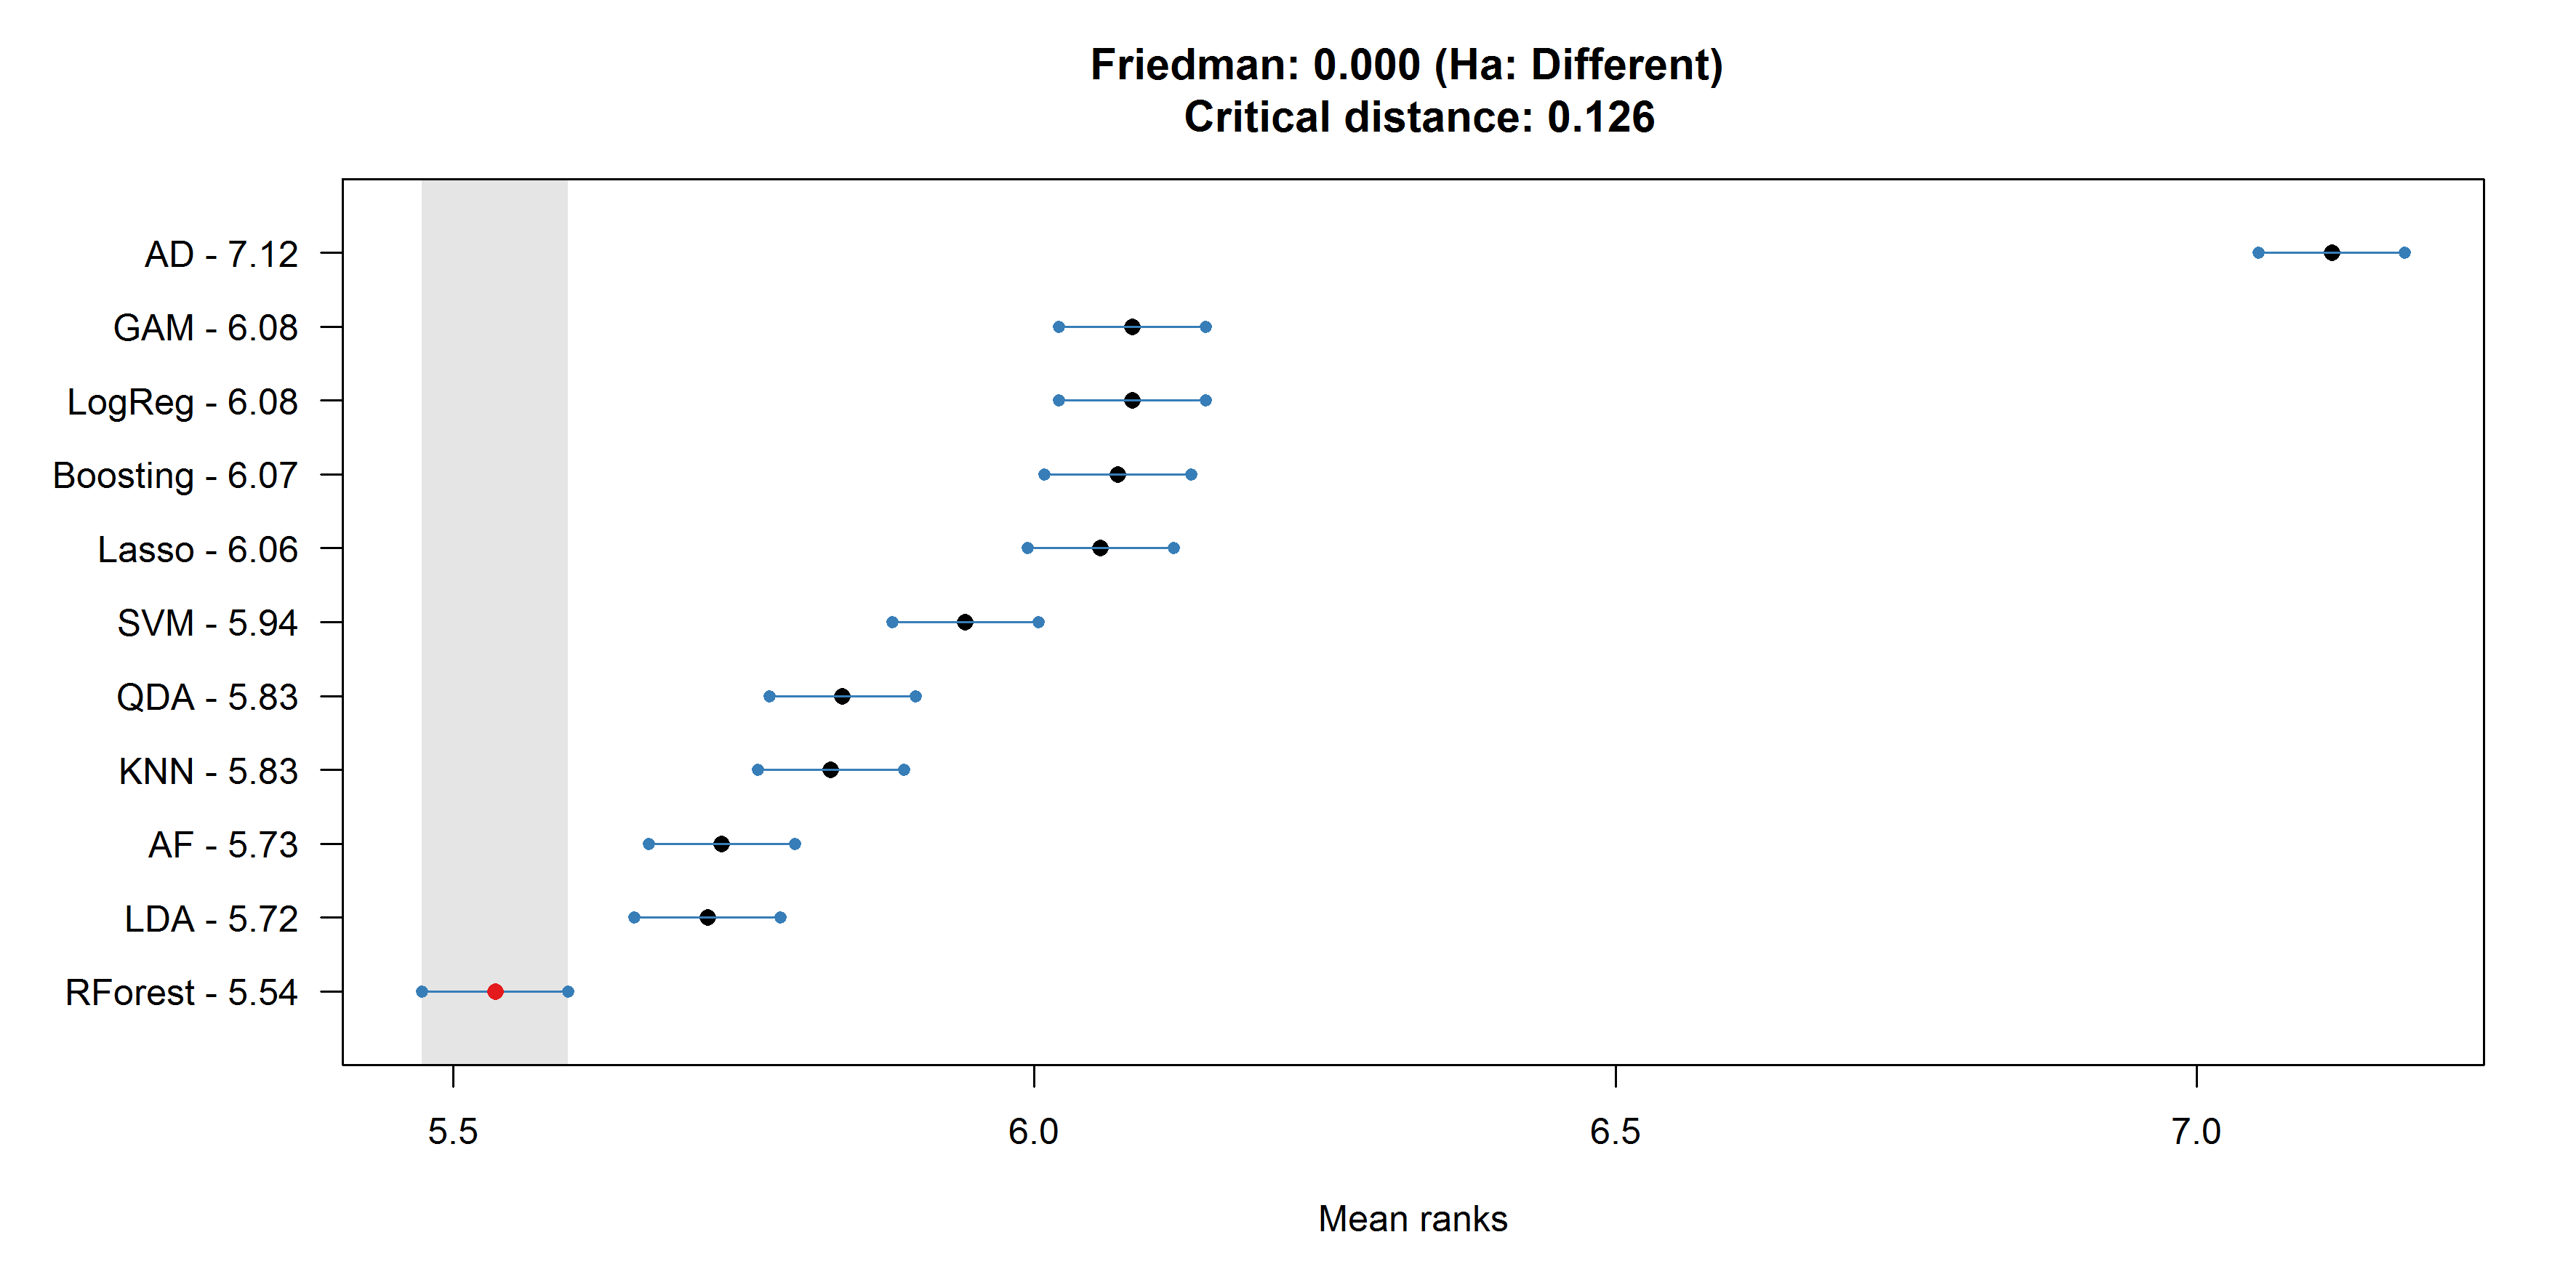
\includegraphics[width=1\linewidth]{img/300dpi/Fig_MCB_all} 

}

\caption{Performance of different models evaluated through MCB test. RMSSE errors are used for computing the ranks and a 95 percentile confidence level.}\label{fig:MCB_ML}
\end{figure}

The Figure \ref{fig:MCB_ML} shows the result of MCB test conducted to
examine the difference between the performance of ML algorithms. The
results shows that there is a statistically significant difference
between the performance RF and all other models. We use AD as a
benchmark, meaning that the approach always predicts AD approach results
in a more accurate forecast for any given time series. According to the
MCB test, AD approach generated the most inaccurate forecasts and
therefore drastically underperformed compared to the others. All other
ML models have much better performance, and the RF comes out as the
ultimate winner in terms of mean rank classification accuracy on the
test data set.

We also perform the utility evaluation of ML models. The results are
presented in the Table \ref{tab:matrix}. The Table \ref{tab:matrix}
represents the average values of RMSSE for AD and AF approaches when the
correct classification was AD and AF, respectively. When the true model
to use is AD (17853 causes), the average RMSSE error is 0.9028 for AD,
and 1.5204 for AF. On the contrary, when the true model to use is AF
(30147 causes), the average RMSSE error is 1.6568 for AD and 0.8669 for
AF. In this way, we design the average costs and benefits associated
with classification decisions and we are able to evaluate the ML models
performances via practical utility measure contribution connected to
their usage, and not just via standard statistical measures. This kind
of performance evaluation has much more value for practitioners
assessing the practical values of each ML model. The presented utility
evaluation can be further extended in practice by linking the monetary
costs to the decision based on the forecast. However, domain knowledge
on the area where forecasts are implemented is required.

\begin{table}
\caption{\label{tab:matrix}Cost and benefit matrix}
\centering
\begin{tabular}[t]{lccc}

\multicolumn{2}{c}{} & \multicolumn{2}{c}{\bf Actual}\\ 
\cline{3-4}
& & AD\  & AF\\
\hline
\multirow{2}{4em}{\bf Predicted} & AD & 0.902872 & 1.6568039\\
& AF & 1.520416 & 0.8669348\\
\hline
\end{tabular}
\end{table}

Figure \ref{fig:tableCB} demonstrates that RF has the smallest utility
metric (cumulative average RMSSE) while performing the classification
task on the test data set. We have also included the Ideal model, a
model that always predict correctly, to highlight the deviation of ML
approaches from this benchmark.

Therefore, the utility metric confirms that RF provides the best choice
for a given time series, bearing in mind that RF has already
demonstrated the best performance according to the classical statistical
measures.

\begin{figure}[H]

{\centering 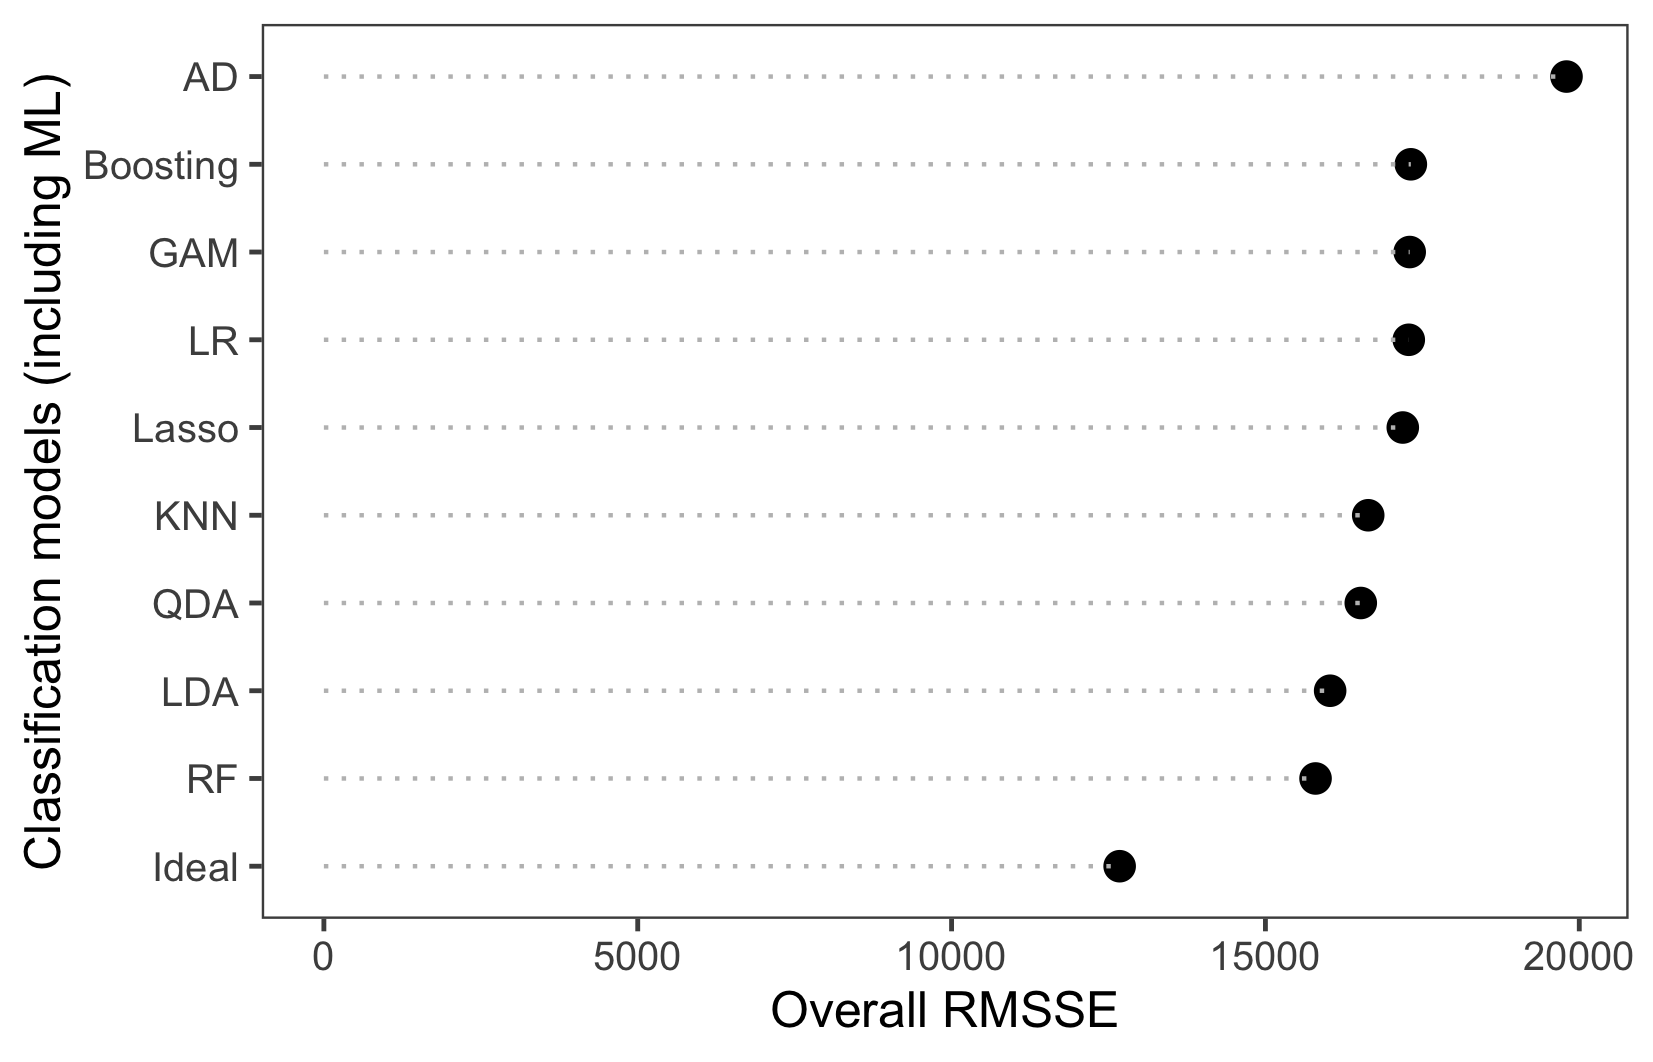
\includegraphics[width=0.6\linewidth]{img/300dpi/utility} 

}

\caption{Utility accuracy comparison}\label{fig:tableCB}
\end{figure}

Among several algorithms, the RF provided the most accurate results
according to the several criteria. Therefore, we further discuss this
approach in the next section in more details.

\hypertarget{building-the-random-forest-algorithm}{%
\subsection{Building the random forest
algorithm}\label{building-the-random-forest-algorithm}}

In this section, we describe building the random Forest. Classification
trees are simple and powerful algorithm, which are often used in
practice for classification supervised learning{[}REF{]}. They are easy
to use, produce accurate predictions, and provide interpreatable
results.

The RF represent the upgraded version of the tree model. The idea behind
the RF is that by averaging individual forecasts from the assembly of
many trees, the variance will be significantly reduced and the final
model will generate a forecast which has low variance and bias as well
{[}REF{]}. The model building process consists of using multiple
bootstrapped random sets of the original data for building the trees
with only a part of the variables included in each individual tree
(Breiman, 1996).

Individually, these trees tend to overfit the data and generate future
forecasts with large variance. But, at the same time, they produce a low
bias. Therefore, in order to reduce the variance, the Bagging process is
building many trees on slightly different train data (since the data is
bootstraped-resampled) and averages forecasts of all the trees in one
unique forecast. For the sake of improving the Bagging process, Breiman
(2001) introduced the RF as an algorithm that mimics the Bagging
process, but uses only a small random sample of the available features,
for building each classification tree. The idea behind this is instead
of just ``shaking'' the data via bootstraped-resampled process, we are
introducing additional randomness in the process by additionally
``shaking'' the features for the forecasting via random sampling of just
part of the features. Therefore, each time a split in a tree is
considered, a random sample of \emph{m} predictors is chosen as a split
candidates from the full set of \emph{p} features. A fresh sample of
\emph{m} features is taken at each split, and typically \emph{m}
\(\approx\) \(\sqrt p\) (Friedman et al., 2001). By forcing this process
each time using the subsample of fresh features, the RF is decorrelating
each tree. In this way, the process of averaging many different trees
will reduce the variance more efficiently than in the case of correlated
trees.

In order to generate the RF model, there are several questions and
tuning parameters that need to be optimized so that the final model
could generate reliable and accurate forecasts. For that purpose,
Friedman et al. (2001) have proposed the following methodology presented
in the Algorithm \ref{alg:RF}.

\begin{algorithm}
    \caption{Random Forest methodology.}
    \begin{algorithmic}[1]
      \item For {$b=1$ to $B$:}
        \begin{enumerate}[label=(\alph*)]
          \item Draw a bootstrap sample \textbf{Z*} of size $N$ from the training data.
          \item Grow a random forest tree $T_b$ to the bootstrapped data, by recursively repeating the following steps for each terminal node of the tree, until the minimum node size $n_{min}$ is reached.
            \begin{enumerate}[label=\roman*]
              \item Select $m$ variables at random from the $p$ variables.
              \item Pick the best variable/split-point among the $m$.
              \item Split the node into two daughter nodes.
            \end{enumerate}
       \end{enumerate}
  \item Output the ensemble of trees $\{T_b\}^B_1$.
    \end{algorithmic}
    \vspace{0.2cm}
    To make a prediction at a new point $x$:\\[0.2cm]
    \textit {Regression}: $\widehat{f}^B_{rf}(x)= \frac{1}{B} \sum_{b=1}^B T_b (x)$.\\[0.2cm]
    \textit {Classification}: Let $\widehat{C}_b(x)$ be the class prediction of the $b$th random-forest tree. \\ 
    \phantom{Classification } Then $\widehat{C}^B_{rf}(x)=majority\;vote\; \{{C}_b(x)\}^B_1$.
    \label{alg:RF}
\end{algorithm}

The first question is how many features to randomly choose for training
in each individual tree (i.e.~tree depth)? The question of how many
trees to use for fitting the RF model emerges also needs to be answered
in parallel. In order to determine the optimal number of features and
trees for building an RF model, the evaluation process is performed with
a different number of features and trees in each split. Therefore, the
resulting process represents the optimization problem of seeking the
minimum of the surface generated by features in each split, trees and
resulting out of the bag (OOB) forecasting error. (Please refer to
Figure \ref{fig:surface}). OOB represents the misclassification error of
the RF model while performing the classification tasks. Also, OOB is the
approximation of the cross validated test error, since the process of
fitting bootstrapped data sets consists from training the model on just
part of the original data and than predicting the remaining part of the
original data (i.e.~out of bag data). By averaging OOB errors from many
different tree models (which comprise the final random forest model),
the final OOB is obtained.

Figure \ref{fig:surface} reveals that increasing number of trees used
for generating RF model that reduces the misclassification error. A
similar scenario is present with a features used in each split, where
increasing the number of features (up to a certain point) reduce
misclassification error. The presented surface is highly erratic and
undulating, making it is hard to visually determine global minimum. For
that reason, the performance of the four best RF models with feature
splits (\emph{m} = 6, 10, 21 and 42) are shown through a different
number of trees used for fitting RF model (Figure \ref{fig:tree_depth}).

The Figure \ref{fig:tree_depth} represents the optimal number of splits
(randomly selected features) used during the process of building each
classification tree, according to OOB forecasting error. As demonstrated
in Figure \ref{fig:tree_depth} the OOB error is minimized on the depth
of 10. Therefore, the optimal number of features (i.e.~tree depth) for
the RF model is \textbf{10}.

\begin{figure}[H]

{\centering 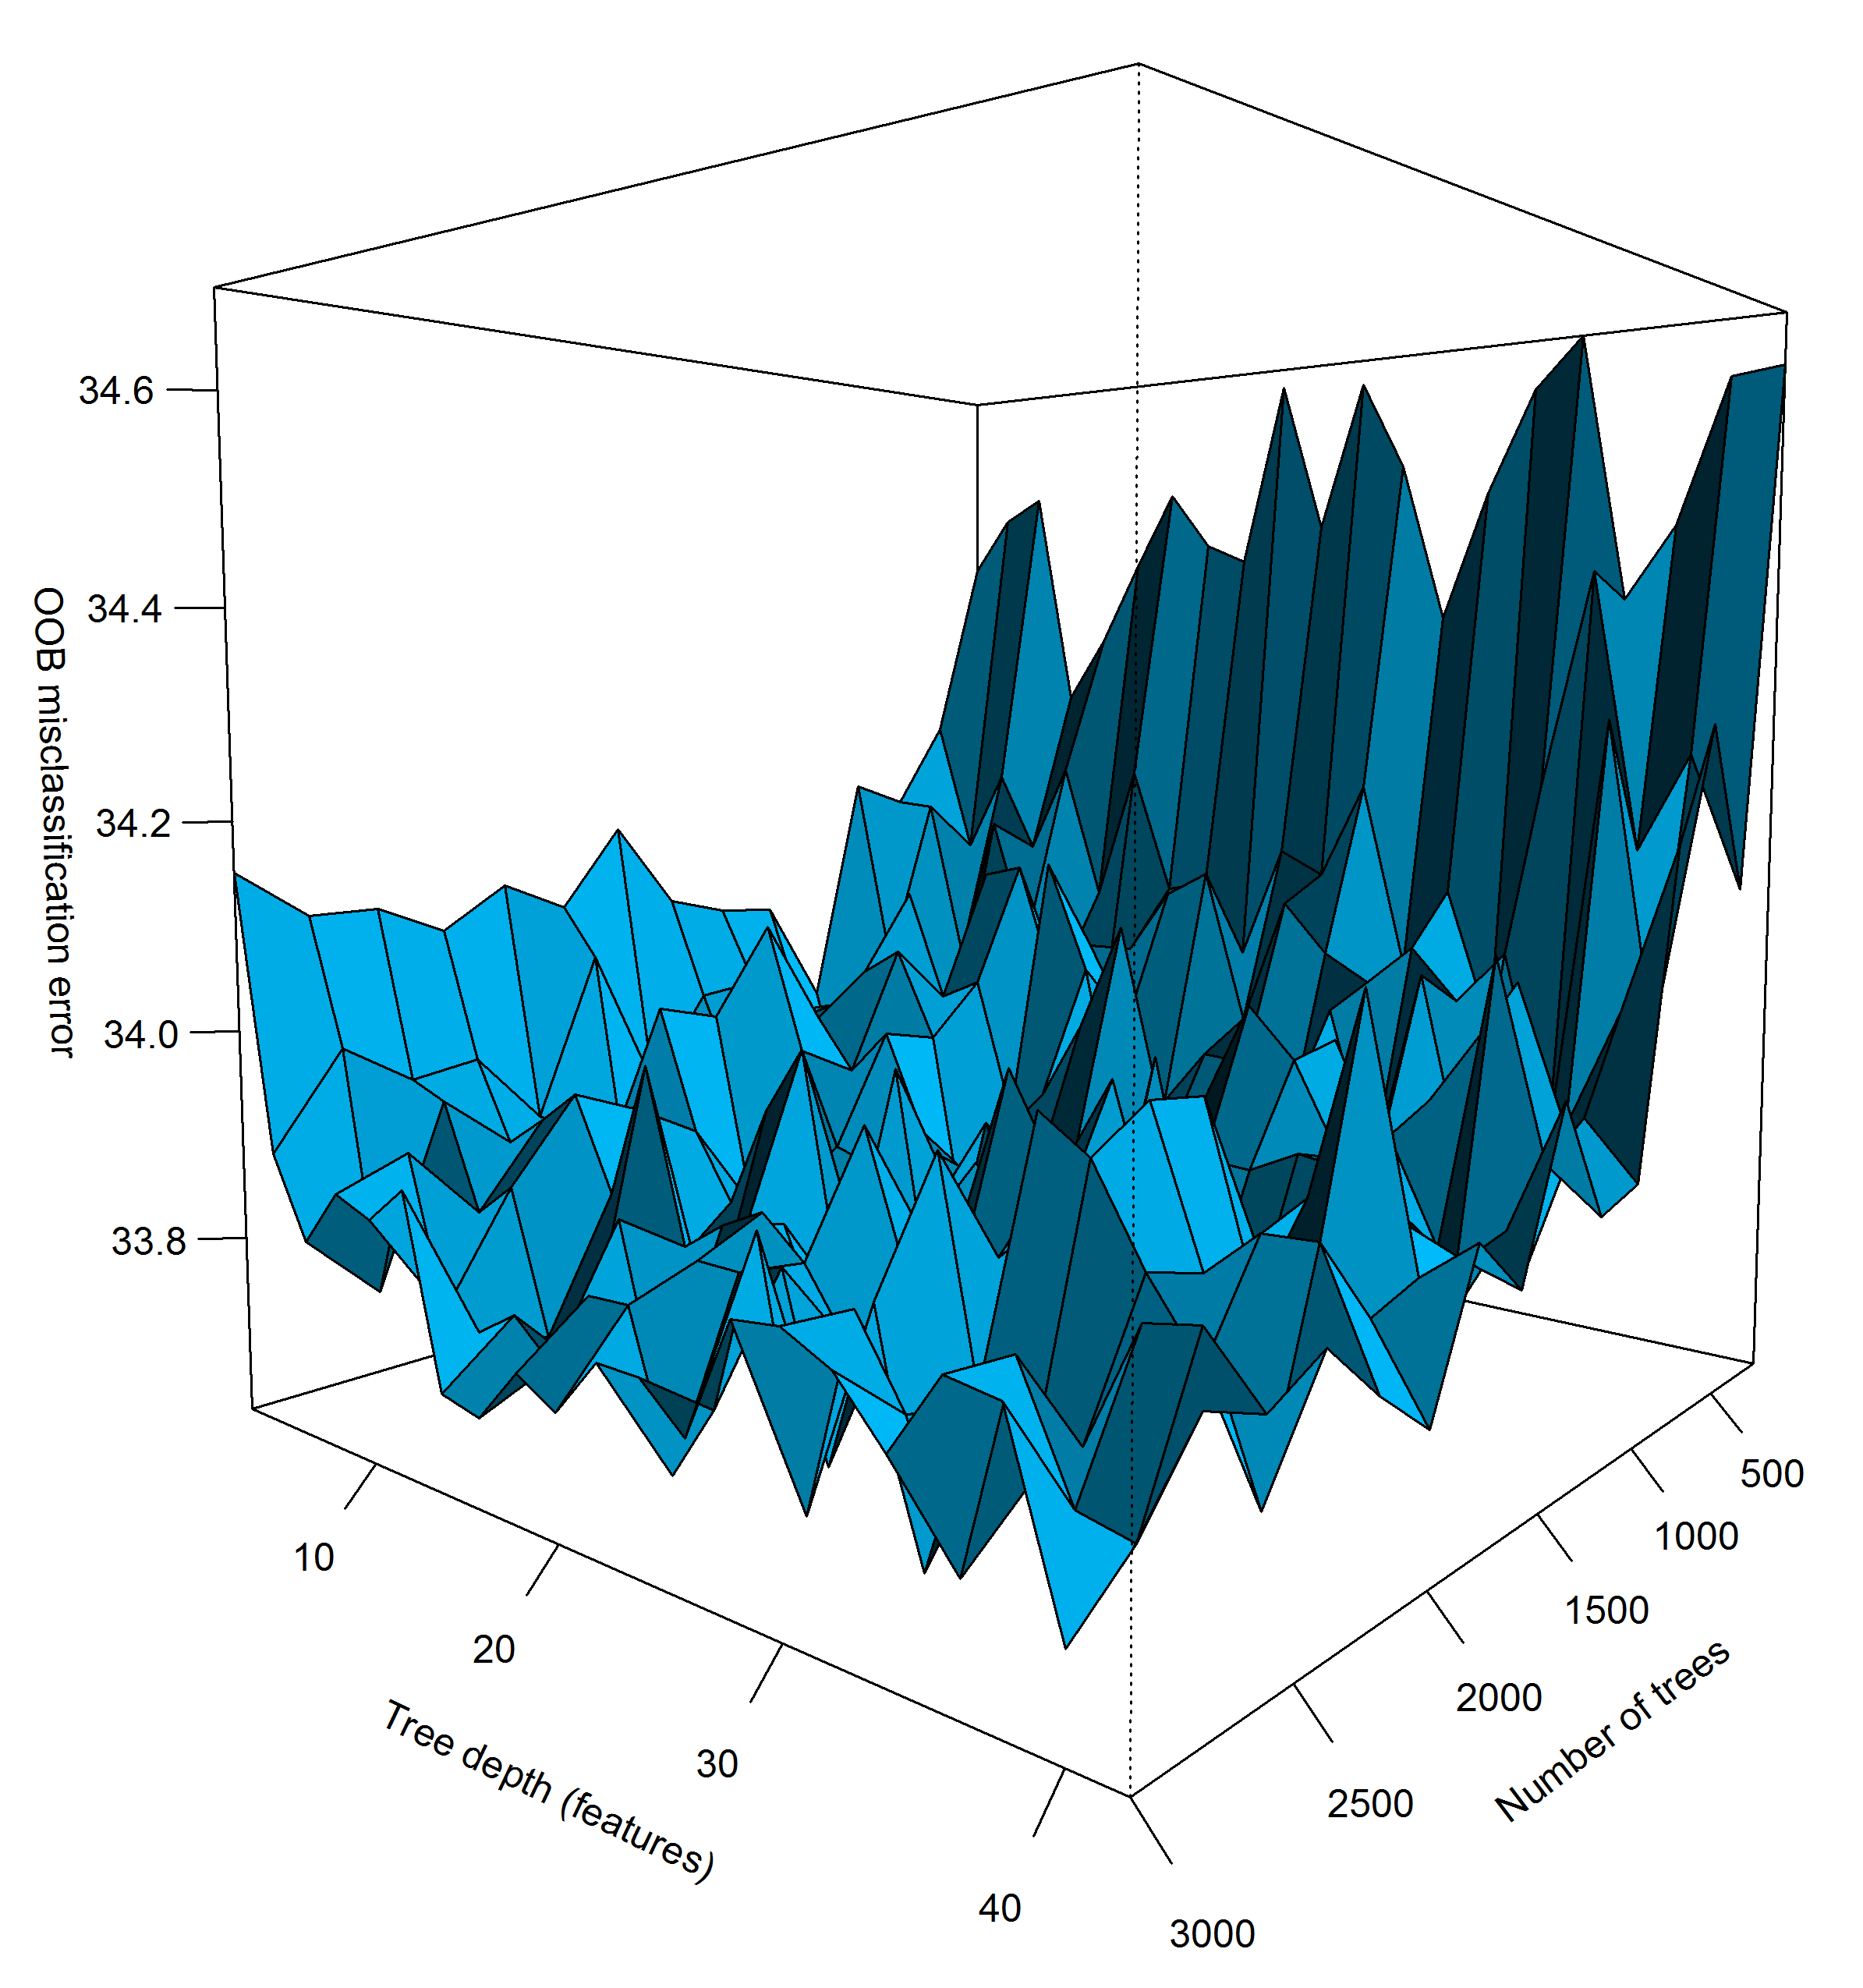
\includegraphics[width=0.7\linewidth]{img/300dpi/Fig_persp} 

}

\caption{Surface plot of the number of features (depth), number of trees and misclassification error of random forest model.}\label{fig:surface}
\end{figure}

The second tuning question is how many trees should be used for
generating the RF model? One of the good merits that help in this
process is RF resilience on the overfitting. Apparently, the averaging
process during RF building appears to be resilient to overfitting
(Friedman et al., 2001). Averaging process during the RF building phase
remedies the negative effects of choosing too large a number of trees
for fitting the model since this will not result in an increase in
variance on the test data set. This implies that the penalty of choosing
a too large number of trees on models' overall performance is minor. The
criteria for this judgment is based on the OOB misclassification error
which the RF model produces on a given data set. Accordingly, the
optimal number of trees is chosen by determining the number of trees
where the OOB misclassification error is stabilized (Figure
\ref{fig:tree_depth}). From Figure \ref{fig:tree_depth} it is clear that
error is stabilized by using the \textbf{3000} trees.

\begin{figure}[H]

{\centering 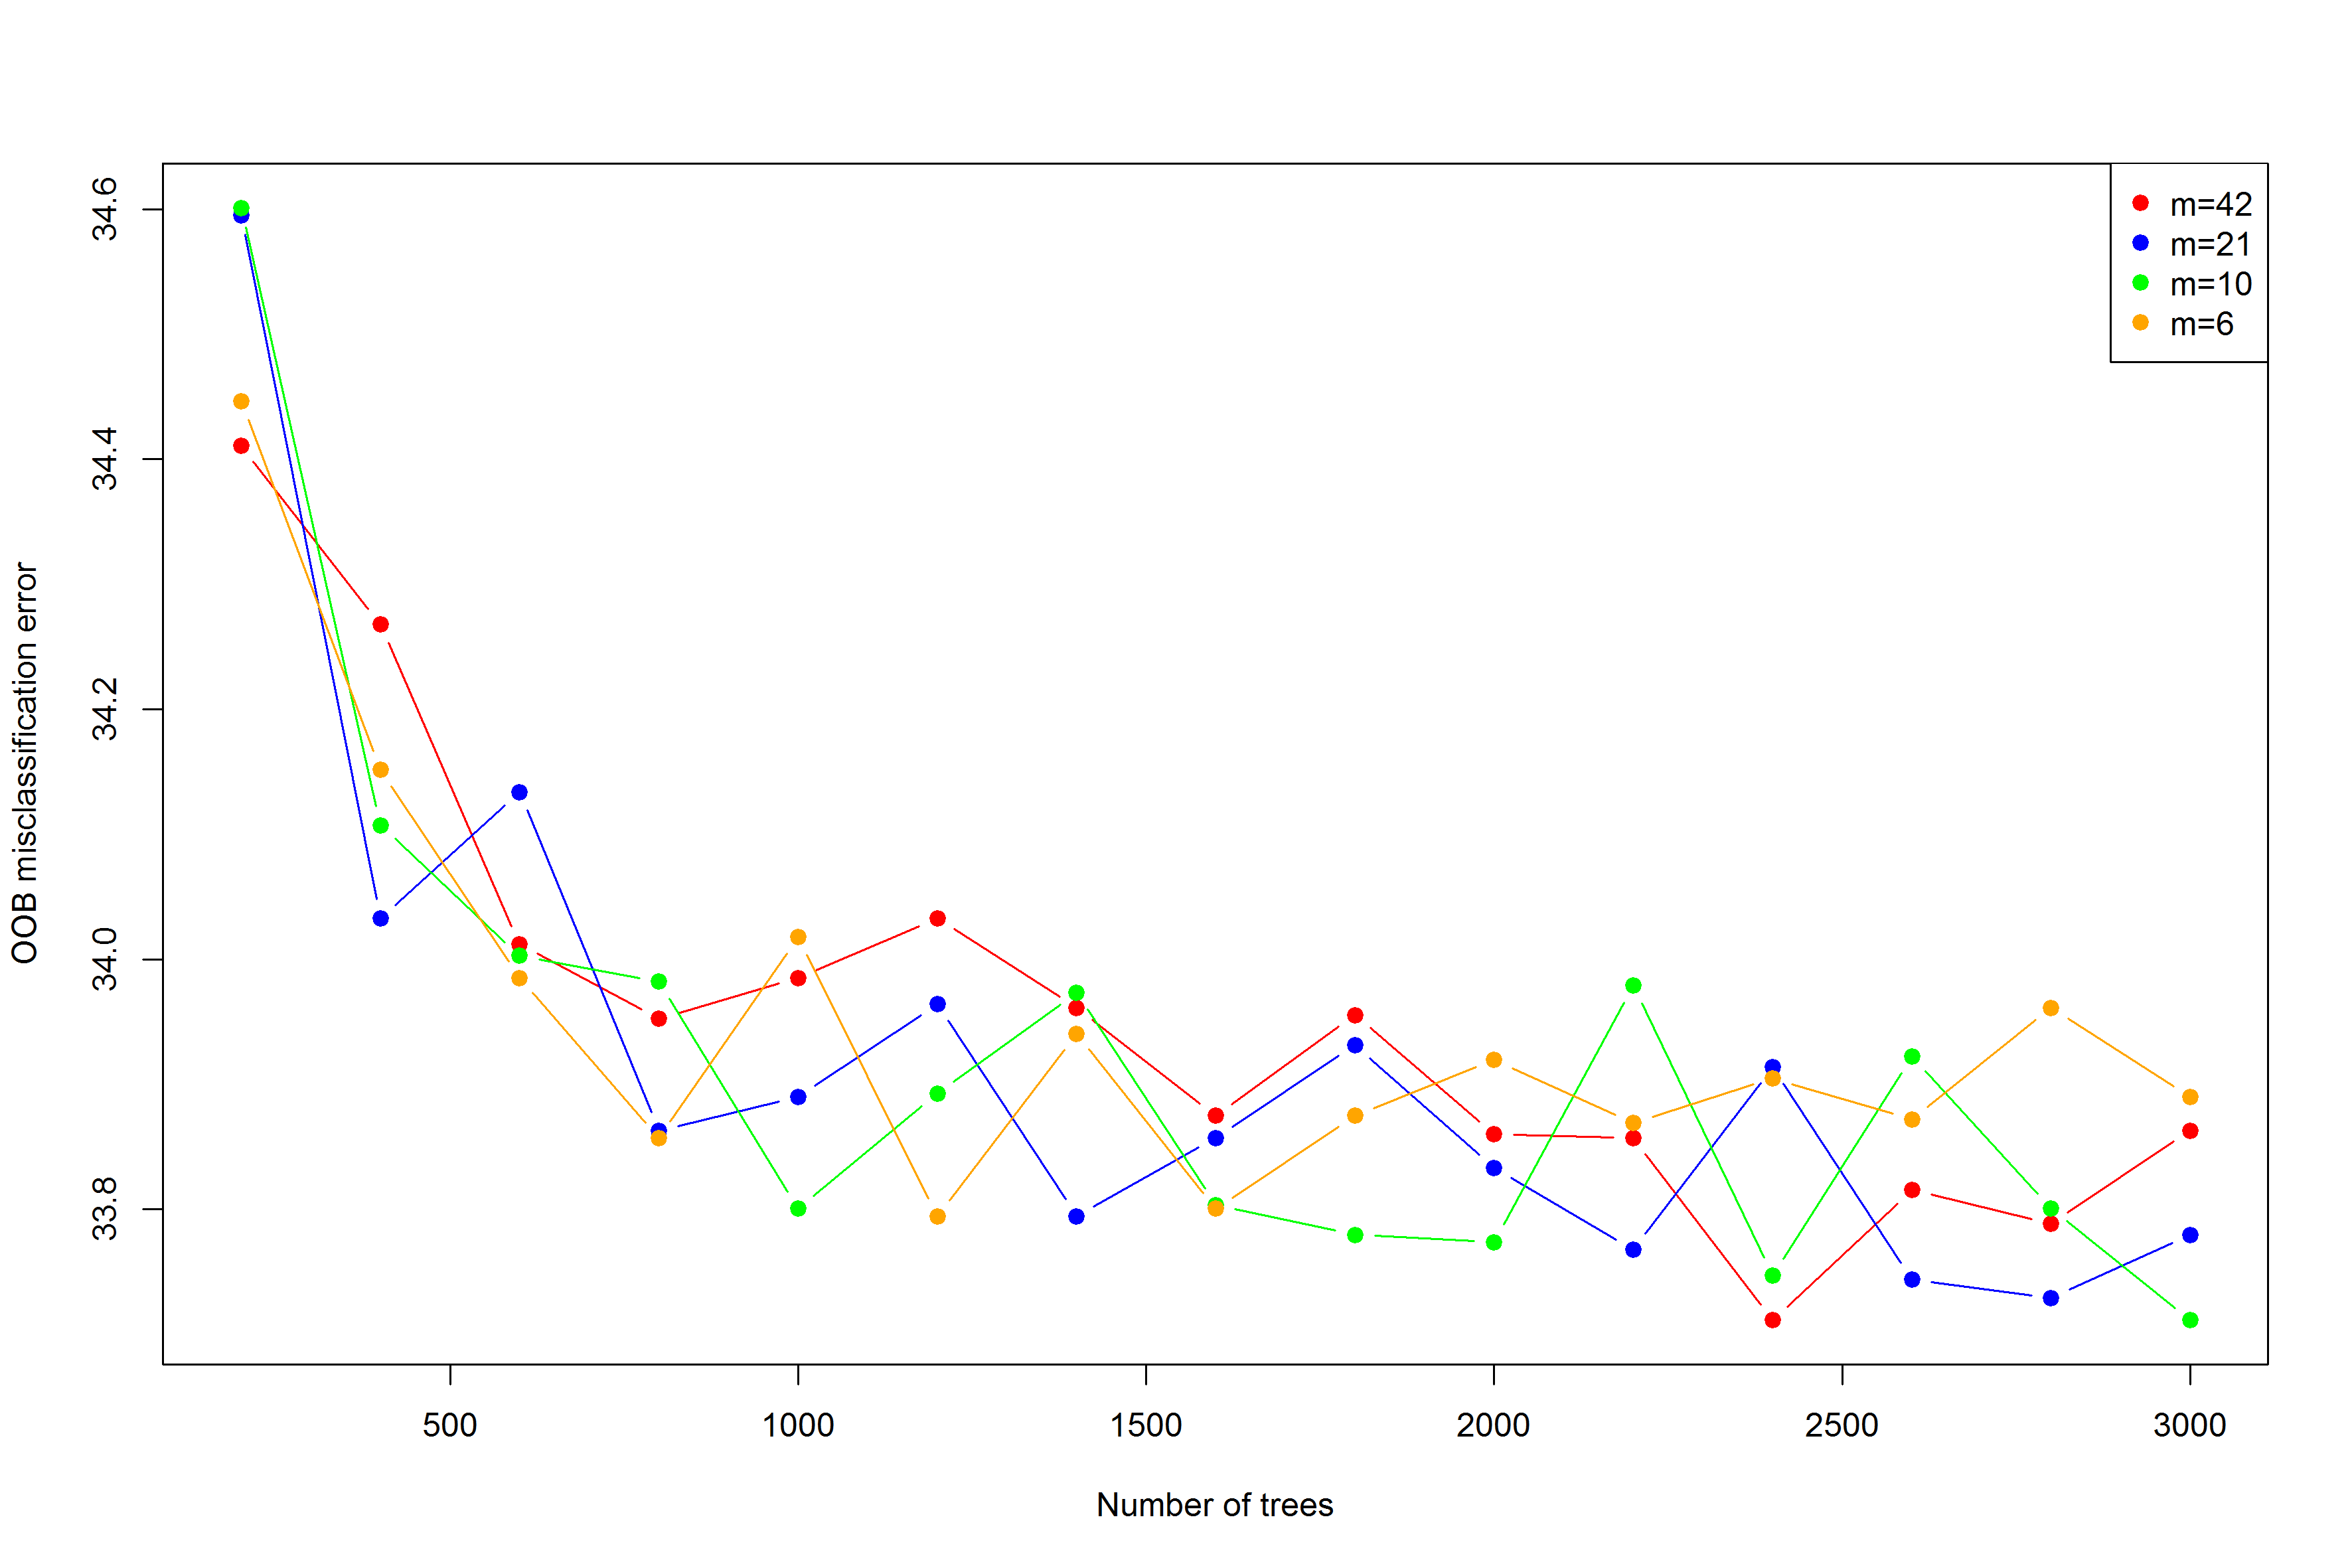
\includegraphics[width=0.9\linewidth]{img/300dpi/Fig_tree_depth_and_ntrees} 

}

\caption{Determining the optimal depth and the of number the trees in the random forest model.}\label{fig:tree_depth}
\end{figure}

\hypertarget{res}{%
\section{Association between time series feasutes and AF/AD
performance}\label{res}}

Since the RF consists of a large number of trees, it is no longer
possible to represent the resulting statistical learning procedure using
a single tree, and it is not clear which variables are most important to
the procedure (James et al., 2013). Therefore, the RF improves
prediction accuracy at the expense of interpretability. Instead, it is
possible to obtain the overall summary of the importance of each feature
by measuring the mean decrease in the Gini index.

\begin{figure}[H]

{\centering 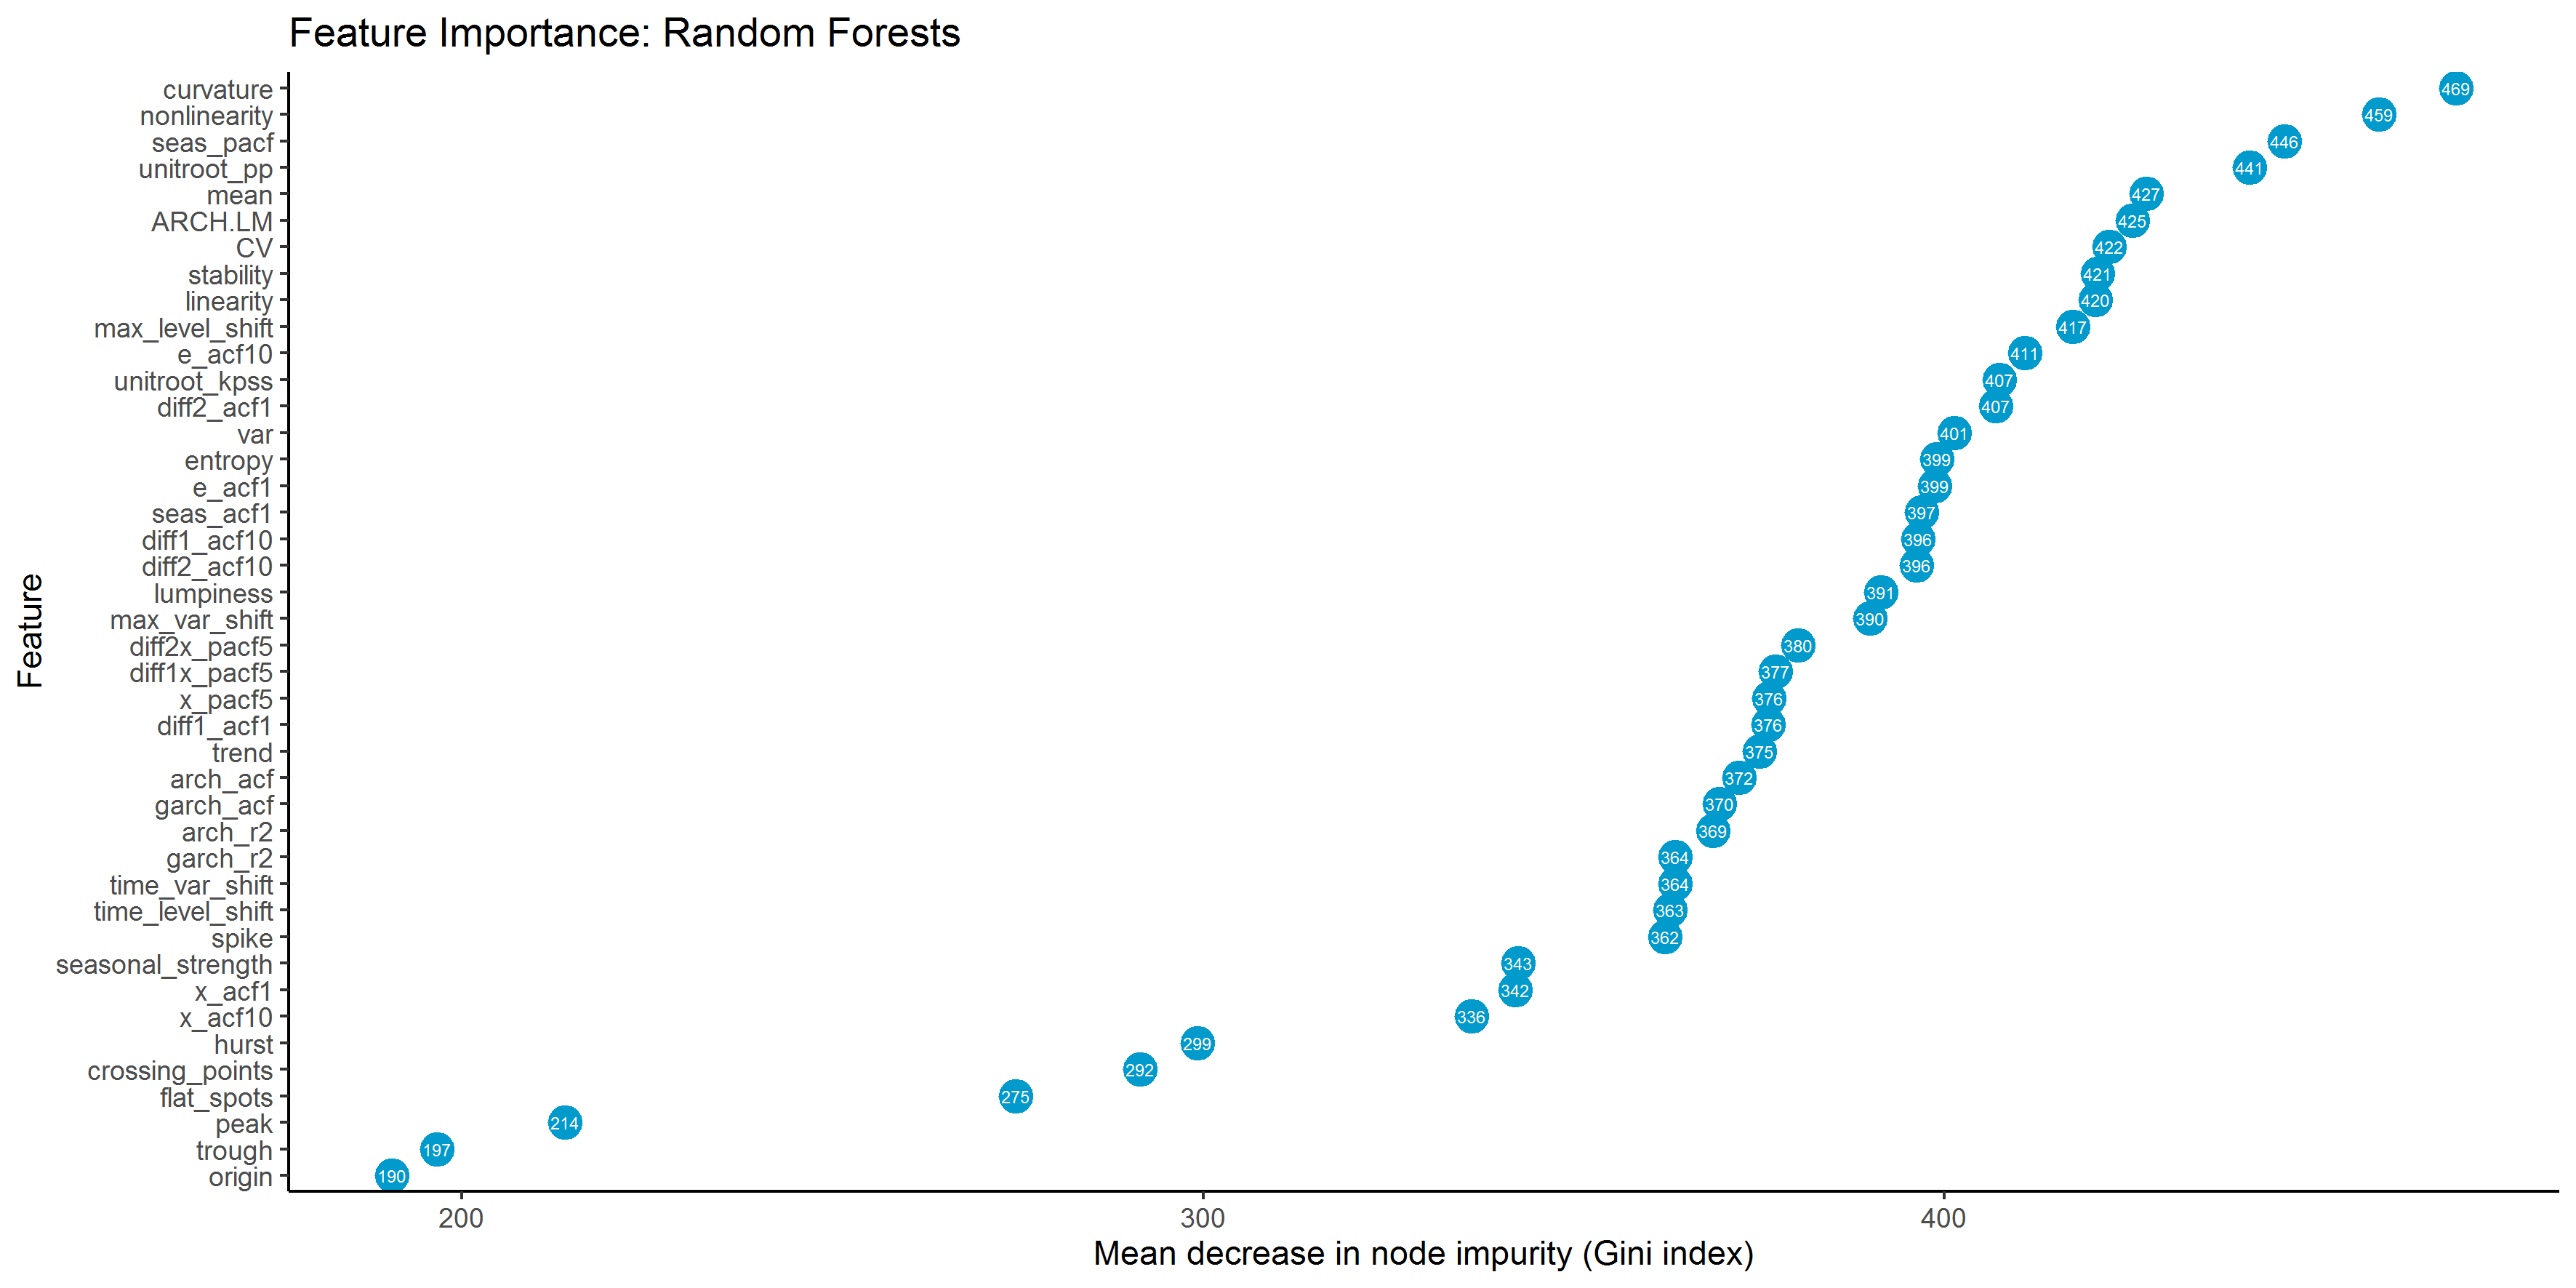
\includegraphics[width=0.95\linewidth]{img/300dpi/Fig_importance} 

}

\caption{Predictor features importance spectrum for the M4 data. A feature importance is computed using the mean decrease in Gini index.}\label{fig:RFpartial}
\end{figure}

The Figure \ref{fig:RFpartial} demonstrates the overall importance of
the features used in building trees during the random successive process
of generating the RF model. Importance of the features is determined by
the decrease in total amount of the node impurity by splits over a given
predictor and averaging over all trees in RF. The decrease of the node
impurity is measured by the Gini index. A large values of the Gini index
indicate the important features. Clearly some features prove to be more
important than others in classifying accurately the AF versus AD
approach. The most important features are: \emph{curvature},
\emph{nonlinearity}, \emph{seas\_pacf}, \emph{unitroot\_up}, \emph{mean}
and \emph{ARCHM.LM}; while \emph{origin}, \emph{through}, \emph{peak}
and \emph{flats spots} seems to be the least important for predicting
which temporal aggregation method to use (AF or AD). The quantity being
modeled here is the probability of correctly choosing the AD versus AF,
and the opposite. The least important features have approximately half
of the importance as the most significant ones. Difference in a decrease
of node impurity from the \emph{curvature} to the \emph{origin} feature
is more than 250 units, indicating the wide range of features
importance.

\begin{figure}[H]

{\centering 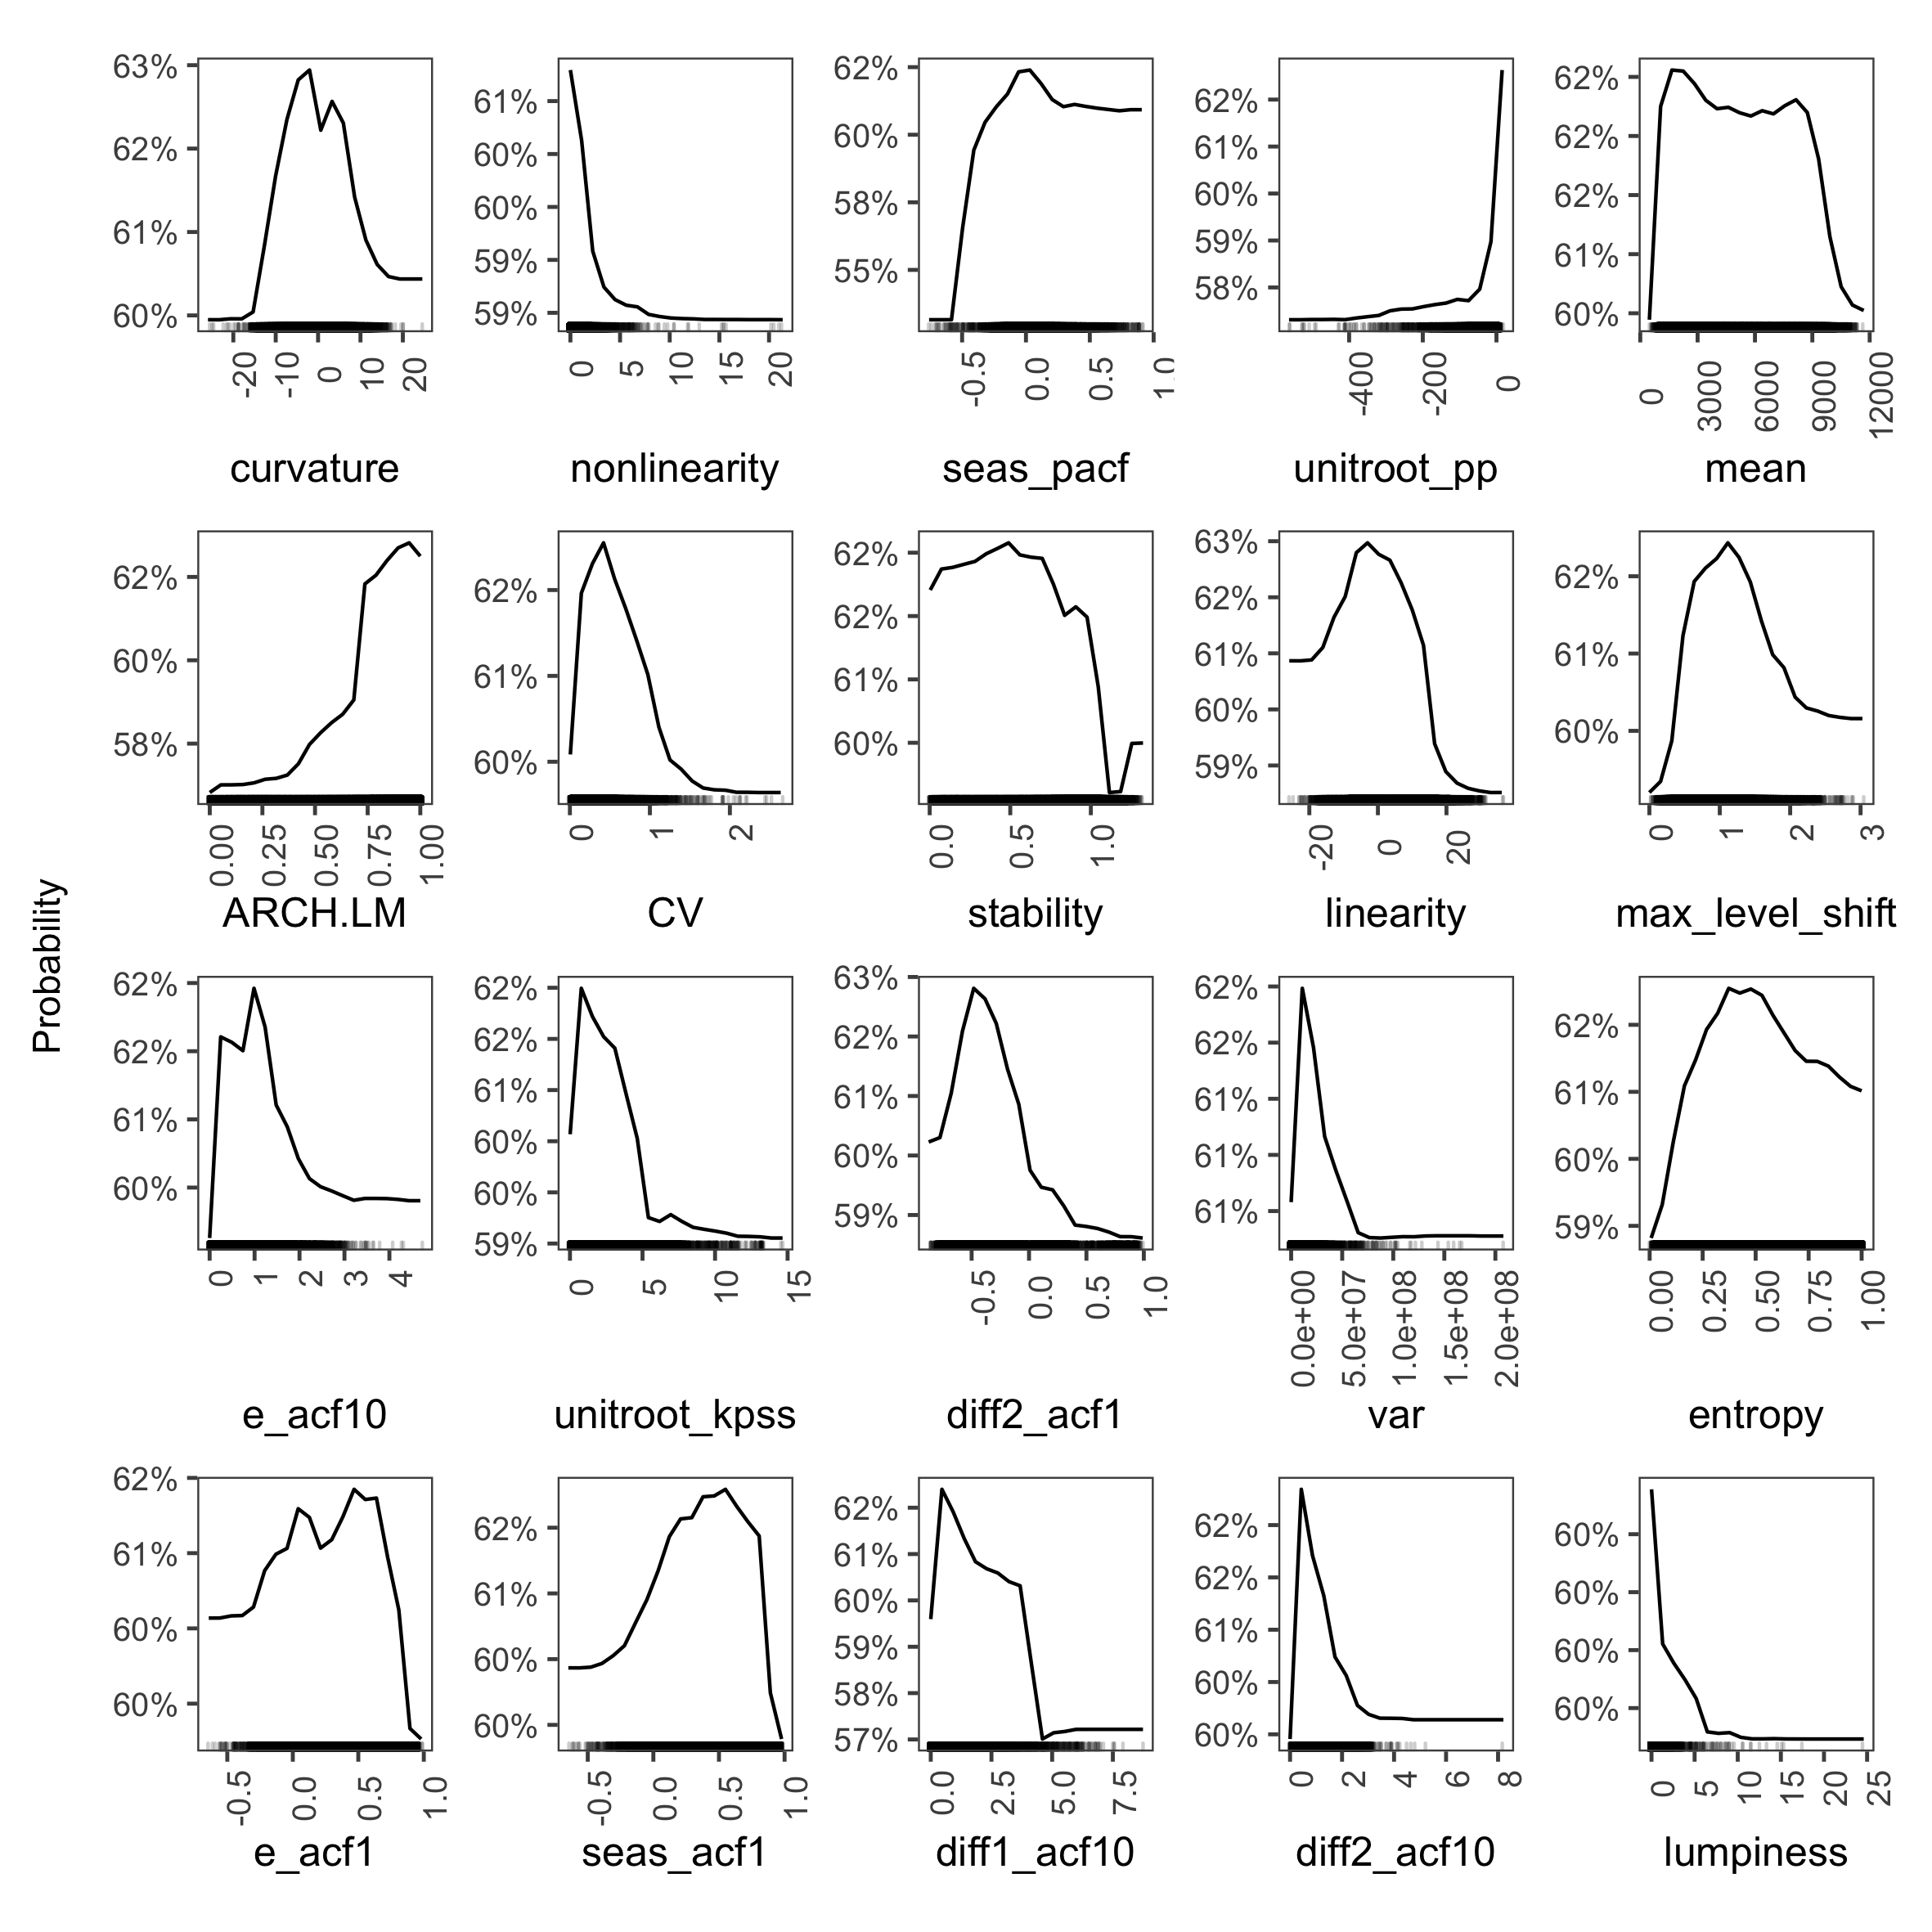
\includegraphics[width=1\linewidth]{img/300dpi/pfinal} 

}

\caption{Partial dependence plots}\label{fig:pdpcommon1}
\end{figure}

\begin{figure}[H]

{\centering 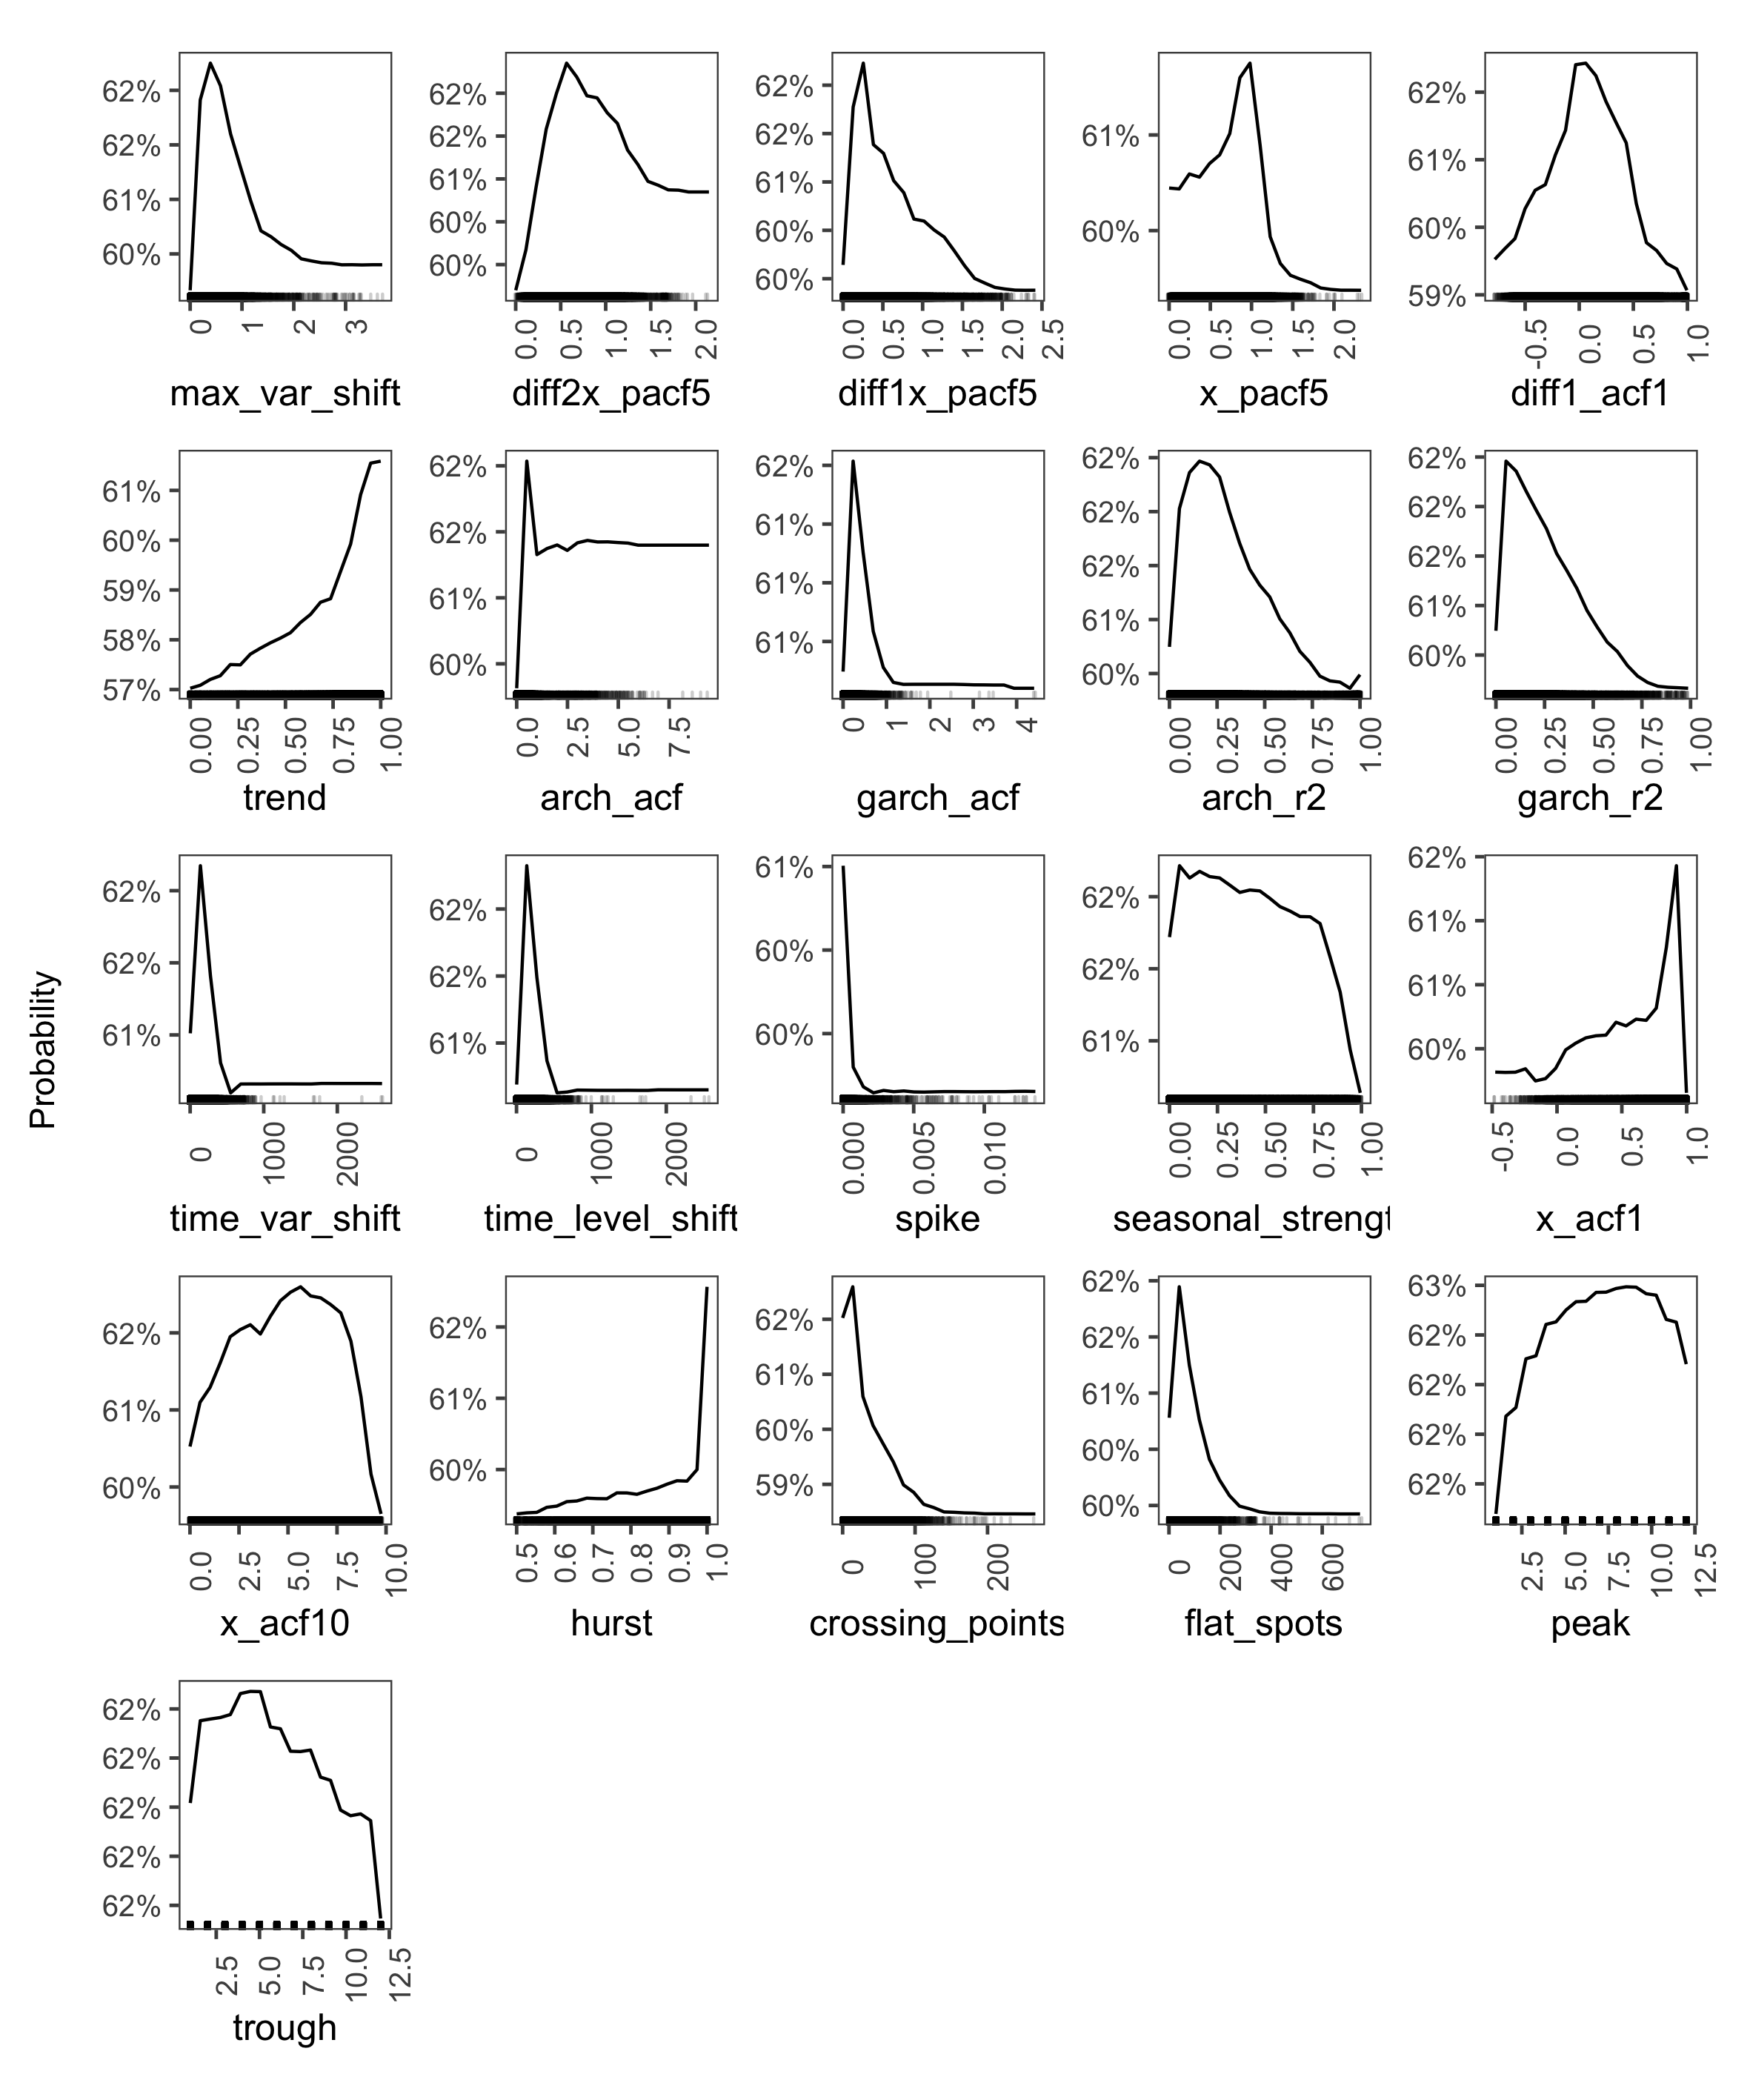
\includegraphics[width=1\linewidth]{img/300dpi/pfinal1} 

}

\caption{Partial dependence plot (continue)}\label{fig:pdpcommon2}
\end{figure}

Figure \ref{fig:pdpcommon1} and \ref{fig:pdpcommon2} represent the
partial dependence plot for all 41 features. The quantity being modeled
here is the probability of classifying AF versus AD. Therefore, the
dependent value is a probability of correctly aggregating forecasts
i.e.~AF approach.

The plots illustrate the marginal effect of the selected features on the
response (outcome) after integrating out all the other variables and
their average effect on the response (James et al., 2013).

The rug marks at the bottom of each plot show the distribution of
feature across the variable range. Note that here the data density is
lower near the edges. This may cause unstable behavior of the curves in
those areas. The vertical scales of the plots show the probability of AF
approach providing more accurate forecast for each feature as values of
that feature changes. It is clear from Figure \ref{fig:pdpcommon1} and
\ref{fig:pdpcommon2} that the features have a mixed effect on the
classifying to the AF and AD approaches. While the efefct might be clear
for feature such as trend or non-linearity, it is less clear for other
such as

We observe that increasing trend, ARCH.LM, hurst, autocorrelation lag 1,
unitroot\_pp and seas\_pacf may increases the chance of AF performing
better, therefore AF become preferable. However, increasing lumpiness,
entropy, no-linearity, curvature, strength of seasonality may increase
the chance of AD performing better, so the strong presence of these
features may favorite AD over AF. It is important to note that we are
less interested in the exact probability in these plots. Instead, we are
interested in discovering how changing time series feature may
increase/decrease the chance of AFor AD Followign the same The rest of
the features

\hypertarget{con}{%
\section{Conclusions}\label{con}}

In time series, the forecast time granularity required to inform a
decision might be different from the time series granularity. For
instance, if a time series is recorded in a higher frequency
(e.g.~monthly), forecast might be required at a lower frequencies
(e.g.~annual). This is very common in modern organisations as data can
be collected in the finest time granularity, such as sub-daily.
Therefore, there are situations where a forecast of the total value over
a time periods ahead (e.g.~horizon aggregation/leadtime) is needed. To
generate such a forecast for a given time series, we may consider two
options: i) First generate forecasts, followed adding them up to obtain
the forecast horizon aggregation (AF), or ii) First aggregate the time
series using non-overlapping temporal aggregation and then and then
generate the forecast (AD). In this paper, we design and execute an
empirical experiment framework using monthly M4 competition data to i)
explore the forecasting performance of these approaches; ii) investigate
the association between time series features and temporal aggregation
approach performance (e.g.~AF or AD).

There is a common assumption that series in the higher level of temporal
aggregation (lower frequency) are smoother with less noise and more
cleaner patterns, which often implies that forecasts created on higher
temporal aggregation levels are more accurate. This practice is usually
may exist in supply chains, where practitioners are usually advised to
aggregate the series to the frequency levels aligned with their decision
making horizons and then to create forecast for the period of interest.
In this paper we questioned this practice and explore the comparative
performance of AF and AD approaches. We conducted a comparative research
of the forecasting performance using 48000 monthly series from M4 data,
at different levels of temporal aggregation corresponding to generating
forecasts at bi-monthly, quarterly, 4--monthly, semi-annual and annual
levels. Results demonstrate that there is a significant number of series
for which aggregate forecast (63\%) outperforms aggregate data (37\%).

Given the fact that there is a lack of rules and indications on which
approach should be used on each time series. We further investigate the
association between time series features and model performance. The need
for such a research investigation has also been highlighted in the
literature (Babai et al., 2021). Therefore, we seek to shed lights on
the effect of temporal aggregation on time series features and further
investigate how they might affect the performance of AD and AF
approaches. To that end, we first construct a database consisting of
features of each time series as predictor and model class labeled as
AF/AD as response/outcome. Then, we build several ML models to
accurately predict the correct class and consequently recommend using
the most accurate approach for a given time series and its features. Our
results show that Random Forest model provide the best performance in
accurately classifying approaches measured through statistical and
utility metrics. Moreover, RF model is used to reveal the most
influencing time series features in resulting in an accurate prediction.
Additionally, We extracted the partial dependence plot to describe a
predictor contribution to the fitted model through a probability and
show that how the value of a feature may favorite AF over AD.

The main findings of this paper can be summarised as follows:

\begin{itemize}
\item
  First of all, when forecasting for the aggregation horizon (leadtime)
  is required, we show that AF is a significantly better methodology to
  use overall. However, the result might be due to the exiting features
  of monthly M4 time series and AF might not be always a better approach
  if features are different such as sub-daily time series. The findings
  indicate that neither of the approaches are always the most accurate
  when the accuracy is reported at the individual time series level. The
  findings clearly show that if a low frequency forecast is required,
  when the time series has a higher frequency, then the most accurate
  forecast is not necessarily generated by non-overlapping temporal
  aggregation. This may call into question the justification of the
  common practice in such a situation.
\item
  Second, non-overlapping temporal aggregation changes the features of
  time series. The magnitude of the change varies for different
  features. In particular, we observe that with increase in the
  aggregation level, the strength of seasonality, the autocorrelation,
  coefficient of variation, linearity, curvature and KPSS unitroot
  statistic decrease. However, non-linearity, mean, variance, ARCH.LM,
  trend , unitroot pp statistics increase. Entropy is the only measure
  that both increases and decreases based on its initial value.
\item
  Third, Random Forest model is the most accurate classifier ML
  algorithm in predicting which approach provides more accurate forecast
  given a set of time series features as input.
\item
  Fourth, RF model revels that the top ten important features for
  predicting whether AF or AD should be used for a given monthly time
  series in M4 competition include \emph{curvature},
  \emph{nonlinearity}, \emph{seas\_pacf}, \emph{unitroot\_up},
  \emph{mean}, \emph{ARCHM.LM}, \emph{Coifficient of Variation},
  \emph{stability}, \emph{linearity} and \emph{max\_level\_shift}.
\item
  Fifth, dependence plots provide some indictions on how time series
  features may favorite AD over AF, vice-versa. We observe that
  increasing seas\_pacf, trend, ARCH.LM, hurst, autocorrelation lag 1
  and unitroot\_pp increases the chance of AF performing better. While,
  increasing Coefficient of Variation, entropy, no-linearity, curvature
  increases the chance of AD performing better, so the strong presence
  of these features may favorite AD over AF.
\end{itemize}

Given the findings of this study and the potential value of temporal
aggregation in time series forecasting, the current study could be
extended in a number of ways. Research into any of the following areas
would prove to be useful:

\begin{itemize}
\item
  The proposed design framework should be replicated with intermittent
  time series, daily and sub-daily time series. Given the features of
  such series, the findings would add value to the current knowledge
  state;
\item
  In this study we use all features to build the ML model, an
  alternative approach would be to use dimension reduction approaches
  for all features representing the same type of information such as
  seasonality, autocorrelation, noise, etc and then build the model;
\item
  The current study only utilises the non-overlapping temporal
  aggregation. Research on how overlapping temporal aggregation affects
  time series features and its connection to forecasting performance
  needs to be investigated;
\item
  Almost all research in the area of temporal aggregation focuses on
  point forecast. Further research is required to investigate the
  connection between time series features and effect of temporal
  aggregation when prediction interval and/or forecast density is
  required;
\item
  The current framework can be extended to examine approaches such as
  MAPA {[}Ref{]} and Temporal hierarchies {[}Ref{]} utilising multiple
  levels of temporal aggregation instead of a single level, and their
  association with time series features;
\item
  A further study could investigate the link between time series
  features and forecast accuracy when forecasts are required at the
  original higher frequency, hence a disaggregation approach should be
  employed.
\end{itemize}

\hypertarget{references}{%
\section*{References}\label{references}}
\addcontentsline{toc}{section}{References}

\hypertarget{refs}{}
\begin{CSLReferences}{1}{0}
\leavevmode\hypertarget{ref-athanasopoulos2017forecasting}{}%
Athanasopoulos, G., Hyndman, R.J., Kourentzes, N., Petropoulos, F.,
2017. Forecasting with temporal hierarchies. European Journal of
Operational Research 262, 60--74.

\leavevmode\hypertarget{ref-athanasopoulos2011tourism}{}%
Athanasopoulos, G., Hyndman, R.J., Song, H., Wu, D.C., 2011. The tourism
forecasting competition. International Journal of Forecasting 27,
822--844.

\leavevmode\hypertarget{ref-babai2012impact}{}%
Babai, M.Z., Ali, M.M., Nikolopoulos, K., 2012. Impact of temporal
aggregation on stock control performance of intermittent demand
estimators: Empirical analysis. Omega 40, 713--721.

\leavevmode\hypertarget{ref-babai2021demand}{}%
Babai, M.Z., Boylan, J.E., Rostami-Tabar, B., 2021. Demand forecasting
in supply chains: A review of aggregation and hierarchical approaches.
International Journal of Production Research 1--25.

\leavevmode\hypertarget{ref-barrow2016distributions}{}%
Barrow, D.K., Kourentzes, N., 2016. Distributions of forecasting errors
of forecast combinations: Implications for inventory management.
International Journal of Production Economics 177, 24--33.

\leavevmode\hypertarget{ref-boylan2016performance}{}%
Boylan, J.E., Babai, M.Z., 2016. On the performance of overlapping and
non-overlapping temporal demand aggregation approaches. International
Journal of Production Economics 181, 136--144.

\leavevmode\hypertarget{ref-breiman1996bagging}{}%
Breiman, L., 1996. Bagging predictors. Machine learning 24, 123--140.

\leavevmode\hypertarget{ref-breiman2001random}{}%
Breiman, L., 2001. Random forests. Machine learning 45, 5--32.

\leavevmode\hypertarget{ref-friedman2001elements}{}%
Friedman, J., Hastie, T., Tibshirani, R., others, 2001. The elements of
statistical learning. Springer series in statistics New York.

\leavevmode\hypertarget{ref-goodwin2018profit}{}%
Goodwin, P., 2018. Profit from your forecasting software: A best
practice guide for sales forecasters. John Wiley \& Sons.

\leavevmode\hypertarget{ref-hyndman2021forecasting}{}%
Hyndman, R.J., Athanasopoulos, G., 2021. Forecasting: Principles and
practice. OTexts.

\leavevmode\hypertarget{ref-hyndman2008automatic}{}%
Hyndman, R.J., Khandakar, Y., 2008. Automatic time series forecasting:
The forecast package for r. Journal of statistical software 27, 1--22.

\leavevmode\hypertarget{ref-hyndman2015large}{}%
Hyndman, R.J., Wang, E., Laptev, N., 2015. Large-scale unusual time
series detection, in: 2015 IEEE International Conference on Data Mining
Workshop (ICDMW). IEEE, pp. 1616--1619.

\leavevmode\hypertarget{ref-james2013introduction}{}%
James, G., Witten, D., Hastie, T., Tibshirani, R., 2013. An introduction
to statistical learning. Springer.

\leavevmode\hypertarget{ref-james2021statistical}{}%
James, G., Witten, D., Hastie, T., Tibshirani, R., 2021. Statistical
learning, in: An Introduction to Statistical Learning. Springer, pp.
15--57.

\leavevmode\hypertarget{ref-jin2015forecasting}{}%
Jin, Y., Williams, B.D., Tokar, T., Waller, M.A., others, 2015.
Forecasting with temporally aggregated demand signals in a retail supply
chain. Journal of Business Logistics 36, 199--211.

\leavevmode\hypertarget{ref-MCB}{}%
Koning, A.J., Franses, P.H., Hibon, M., Stekler, H.O., 2005. The M3
competition: Statistical tests of the results. International Journal of
Forecasting 21, 397--409.

\leavevmode\hypertarget{ref-kourentzes2015forecasting}{}%
Kourentzes, N., Petropoulos, F., 2016. Forecasting with multivariate
temporal aggregation: The case of promotional modelling. International
Journal of Production Economics 181, 145--153.

\leavevmode\hypertarget{ref-kourentzes2014improving}{}%
Kourentzes, N., Petropoulos, F., Trapero, J.R., 2014. Improving
forecasting by estimating time series structural components across
multiple frequencies. International Journal of Forecasting 30, 291--302.

\leavevmode\hypertarget{ref-kourentzes2014improving}{}%
Kourentzes, N., Petropoulos, F., Trapero, J.R., 2014. Improving
forecasting by estimating time series structural components across
multiple frequencies. International Journal of Forecasting 30, 291--302.

\leavevmode\hypertarget{ref-kourentzes2017demand}{}%
Kourentzes, N., Rostami-Tabar, B., Barrow, D.K., 2017. Demand
forecasting by temporal aggregation: Using optimal or multiple
aggregation levels? Journal of Business Research 78, 1--9.

\leavevmode\hypertarget{ref-kourentzes2017demand}{}%
Kourentzes, N., Rostami-Tabar, B., Barrow, D.K., 2017. Demand
forecasting by temporal aggregation: Using optimal or multiple
aggregation levels? Journal of Business Research 78, 1--9.

\leavevmode\hypertarget{ref-luna2011top}{}%
Luna, I., Ballini, R., 2011. Top-down strategies based on adaptive fuzzy
rule-based systems for daily time series forecasting. International
Journal of Forecasting 27, 708--724.

\leavevmode\hypertarget{ref-Makridakis2018}{}%
Makridakis, S., 2018. M4 competitor's guide: Prizes and rules.
University of Nicosia.

\leavevmode\hypertarget{ref-mircetic2021forecasting}{}%
Mircetic, D., Rostami-Tabar, B., Nikolicic, S., Maslaric, M., 2021.
Forecasting hierarchical time series in supply chains: An empirical
investigation. International Journal of Production Research 1--20.

\leavevmode\hypertarget{ref-mohammadipour2012forecast}{}%
Mohammadipour, M., Boylan, J.E., 2012. Forecast horizon aggregation in
integer autoregressive moving average (INARMA) models. Omega 40,
703--712.

\leavevmode\hypertarget{ref-nikolopoulos2021we}{}%
Nikolopoulos, K., 2021. We need to talk about intermittent demand
forecasting. European Journal of Operational Research 291, 549--559.

\leavevmode\hypertarget{ref-nikolopoulos2011aggregate}{}%
Nikolopoulos, K., Syntetos, A.A., Boylan, J.E., Petropoulos, F.,
Assimakopoulos, V., 2011. An aggregate--disaggregate intermittent demand
approach ({ADIDA}) to forecasting: An empirical proposition and
analysis. Journal of the Operational Research Society 62, 544--554.

\leavevmode\hypertarget{ref-nikolopoulos2011aggregate}{}%
Nikolopoulos, K., Syntetos, A.A., Boylan, J.E., Petropoulos, F.,
Assimakopoulos, V., 2011. An aggregate--disaggregate intermittent demand
approach ({ADIDA}) to forecasting: An empirical proposition and
analysis. Journal of the Operational Research Society 62, 544--554.

\leavevmode\hypertarget{ref-petropoulos2022forecasting}{}%
Petropoulos, F., Apiletti, D., Assimakopoulos, V., Babai, M.Z., Barrow,
D.K., Taieb, S.B., Bergmeir, C., Bessa, R.J., Bijak, J., Boylan, J.E.,
others, 2022. Forecasting: Theory and practice. International Journal of
Forecasting.

\leavevmode\hypertarget{ref-petropoulos2014forecast}{}%
Petropoulos, F., Kourentzes, N., 2014. Forecast combinations for
intermittent demand. Journal of the Operational Research Society 66,
914--924.

\leavevmode\hypertarget{ref-petropoulos2015forecast}{}%
Petropoulos, F., Kourentzes, N., 2015. Forecast combinations for
intermittent demand. Journal of the Operational Research Society 66,
914--924.

\leavevmode\hypertarget{ref-rossana1995temporal}{}%
Rossana, R.J., Seater, J.J., 1995. Temporal aggregation and economic
time series. Journal of Business \& Economic Statistics 13, 441--451.

\leavevmode\hypertarget{ref-rostami2019impact}{}%
Rostami-Tabar, B., Babai, M.Z., Ali, M., Boylan, J.E., 2019. The impact
of temporal aggregation on supply chains with ARMA (1, 1) demand
processes. European Journal of Operational Research 273, 920--932.

\leavevmode\hypertarget{ref-rostami2021aggregate}{}%
Rostami-Tabar, B., Babai, M.Z., Syntetos, A., 2021. To aggregate or not
to aggregate: Forecasting of finite autocorrelated demand. arXiv
preprint arXiv:2103.16310.

\leavevmode\hypertarget{ref-rostami2013demand}{}%
Rostami-Tabar, B., Babai, M.Z., Syntetos, A., Ducq, Y., 2013. Demand
forecasting by temporal aggregation. Naval Research Logistics (NRL) 60,
479--498.

\leavevmode\hypertarget{ref-rostami2013demand}{}%
Rostami-Tabar, B., Babai, M.Z., Syntetos, A., Ducq, Y., 2013. Demand
forecasting by temporal aggregation. Naval Research Logistics (NRL) 60,
479--498.

\leavevmode\hypertarget{ref-rostami2014note}{}%
Rostami-Tabar, B., Babai, M.Z., Syntetos, A., Ducq, Y., 2014. A note on
the forecast performance of temporal aggregation. Naval Research
Logistics (NRL) 61, 489--500.

\leavevmode\hypertarget{ref-rostami2014note}{}%
Rostami-Tabar, B., Babai, M.Z., Syntetos, A., Ducq, Y., 2014. A note on
the forecast performance of temporal aggregation. Naval Research
Logistics (NRL) 61, 489--500.

\leavevmode\hypertarget{ref-rostami2020anticipating}{}%
Rostami-Tabar, B., Ziel, F., 2020. Anticipating special events in
emergency department forecasting. International Journal of Forecasting.

\leavevmode\hypertarget{ref-Spiliotis2020}{}%
Spiliotis, E., Kouloumos, A., Assimakopoulos, V., Makridakis, S., 2020.
Are forecasting competitions data representative of the reality?
International Journal of Forecasting 36, 37--53.

\leavevmode\hypertarget{ref-spithourakis2011improving}{}%
Spithourakis, G.P., Petropoulos, F., Babai, M.Z., Nikolopoulos, K.,
Assimakopoulos, V., 2011. Improving the performance of popular supply
chain forecasting techniques. Supply Chain Forum: an international
journal 12, 16--25.

\leavevmode\hypertarget{ref-wang2009rule}{}%
Wang, X., Smith-Miles, K., Hyndman, R., 2009. Rule induction for
forecasting method selection: Meta-learning the characteristics of
univariate time series. Neurocomputing 72, 2581--2594.

\leavevmode\hypertarget{ref-wei1978some}{}%
Wei, W.W., 1978. Some consequences of temporal aggregation in seasonal
time series models, in: Seasonal Analysis of Economic Time Series. NBER,
pp. 433--448.

\leavevmode\hypertarget{ref-willemain1994forecasting}{}%
Willemain, T.R., Smart, C.N., Shockor, J.H., DeSautels, P.A., 1994.
Forecasting intermittent demand in manufacturing: A comparative
evaluation of croston's method. International Journal of forecasting 10,
529--538.

\leavevmode\hypertarget{ref-zotteri2007model}{}%
Zotteri, G., Kalchschmidt, M., 2007. A model for selecting the
appropriate level of aggregation in forecasting processes. International
Journal of Production Economics 108, 74--83.

\end{CSLReferences}


\end{document}
